\documentclass[12pt, a4paper]{article}

\usepackage[version=3]{mhchem} 
\usepackage{siunitx} 
\usepackage{graphicx,wrapfig} 
\usepackage{natbib} 
\usepackage{amsmath} 
\usepackage{titling}
\usepackage{setspace}
\usepackage{geometry}
\usepackage{enumitem}
\usepackage{graphicx}
\usepackage{tabularx}
\usepackage{textcomp}
\usepackage{siunitx}
\usepackage{listings}
\usepackage{color}
\usepackage{endnotes}
\usepackage[utf8]{inputenc}
\usepackage{cochineal}
\usepackage[T1]{fontenc}
\usepackage{amsfonts}
\usepackage{fancyhdr}
\usepackage{amssymb}
\usepackage{xcolor} 
\usepackage{mdframed}
\usepackage{multirow}
\usepackage{multicol} 
\usepackage{tikz}
\usepackage[absolute]{textpos} 
\usepackage{colortbl}
\usepackage{array}
\usepackage{geometry}
\usepackage{fancyhdr}
\usepackage[english, vietnamese]{babel}
\usepackage[export]{adjustbox}
\usepackage{indentfirst}
\usepackage{multirow}
\usepackage{float}
\usepackage{listings}
\usepackage{blindtext}
\usepackage{subfig}
\usepackage[figuresleft]{rotating}
\usepackage{afterpage}
\usepackage{witharrows}
\usepackage{framed}
\usepackage[makeroom]{cancel}
\usepackage{mathtools}
\usepackage{adjustbox}
\usepackage{kbordermatrix}
\usepackage{etoolbox}
\usepackage{helvet}
\usepackage{ragged2e}
\usepackage[explicit]{titlesec}
\usepackage{shadowtext}
\usepackage{longtable}
\definecolor{myBlue}{HTML}{0088FF}
\makeatletter

\usepackage{amsthm}
\definecolor{amber}{rgb}{1.0, 0.49, 0.0}
\definecolor{cadmiumgreen}{rgb}{0.0, 0.42, 0.24}
\definecolor{codegreen}{rgb}{0,0.6,0}
\definecolor{codegray}{rgb}{0.5,0.5,0.5}
\definecolor{codepurple}{rgb}{0.58,0,0.82}
\definecolor{backcolour}{rgb}{0.95,0.95,0.92}

\patchcmd{\l@section}
{\hfil}
{\leaders\hbox{\normalfont$\m@th\mkern \@dotsep mu\hbox{.}\mkern \@dotsep mu$}\hfill}
{}{}
\makeatother


\DeclarePairedDelimiter\ceil{\lceil}{\rceil}
\DeclarePairedDelimiter\floor{\lfloor}{\rfloor}
\usetikzlibrary{matrix,calc}
\usetikzlibrary{arrows}


\renewenvironment{leftbar}{%
  \def\FrameCommand{{\color{myyellow}\vrule width 2pt depth 6pt} \hspace{10pt}}%
  \MakeFramed {\advance\hsize-\width \FrameRestore}}%
 {\endMakeFramed}

\newgeometry{
	a4paper,
	left=19.1mm,
	right=19.1mm,
	top=25.4mm,
	bottom=25.4mm,
}


\geometry{
	textheight=100ex,
	textwidth=40em,
	top=30pt,
	headheight=30pt,
	headsep=22pt,
	inner=80pt}

\pagestyle{fancy}
\fancyhf{}
\renewcommand{\headrulewidth}{.4pt}
\renewcommand{\footrulewidth}{.4pt}
\fancyhead[L]{
  \rule[-0.2\baselineskip]{0pt}{0pt}
  
\includegraphics[height=2.2\baselineskip,valign=c]{Logo-BK}
  \fontfamily{ppl}\fontseries{m}\fontsize{12}{10}\selectfont
 	\begin{tabular}{l}
      Restaurant Point-of-sale \\[1.2mm] System Design
   	\end{tabular}
}

\setlength{\headheight}{3.5\baselineskip}

\rfoot{\thepage}

\lfoot{\fontfamily{ccr}\fontseries{m}\fontsize{11.4}{10}\selectfont \textit{Software Engineering (CO3001)}}

\renewcommand\thesection{\arabic{section}}
\renewcommand\thesubsection{\thesection.\arabic{subsection}}


\newlength{\Oldarrayrulewidth}
\newcommand{\Cline}[2]{%
  \noalign{\global\setlength{\Oldarrayrulewidth}{\arrayrulewidth}}%
  \noalign{\global\setlength{\arrayrulewidth}{#1}}\cline{#2}%
  \noalign{\global\setlength{\arrayrulewidth}{\Oldarrayrulewidth}}}


\lstdefinestyle{mystyle}{
	frame=tb,
	language=Python,
    backgroundcolor=\color{backcolour},   
    commentstyle=\color{codegreen},
    keywordstyle=\color{blue},
    numberstyle=\footnotesize\color{gray}\ttfamily,
    stringstyle=\color{codepurple},
    basicstyle=\fontfamily{cmtt}\fontseries{m}\fontsize{11}{10}\selectfont,
    breakatwhitespace=false,         
    breaklines=true,                 
    captionpos=b,                    
    keepspaces=true,                 
    numbers=left,                    
    numbersep=5pt,                  
    showspaces=false,                
    showstringspaces=false,
    showtabs=false,                  
    tabsize=2
}

\lstset{style=mystyle}

\renewcommand{\thesubfigure}{Figure \arabic{subfigure}}
\captionsetup[subfigure]{labelformat=simple, labelsep=colon}

\addto\captionsvietnamese{
  \renewcommand{\contentsname}{Table of Contents}
  \renewcommand{\figurename}{Figure}
}


\newcounter{bluesection}

\renewcommand{\kbldelim}{[}
\renewcommand{\kbrdelim}{]}

\newcommand*{\bluechaperstyle}{
\titleformat{name=\section, numberless}[hang]{\LARGE\bfseries\sffamily}%
{\rlap{\color{myBlue}\rule[-6pt]{0mm}{1.2pt}}\colorbox{myBlue}{%
		\raisebox{0pt}[25pt][12pt]{ \makebox[53pt]{% height, width
				\fontfamily{phv}\selectfont\color{white}{\refstepcounter{bluesection}\Alph{bluesection}}}
}}}%
{15pt}%
{ \color{myBlue}##1
	%
}
\titlespacing*{name=\section, numberless}{-25mm}{3mm}{5mm}
}

\newcommand*{\bluechaperNONUM}{
	\titleformat{name=\section, numberless}[hang]{\LARGE\bfseries\sffamily}%
	{\rlap{\color{myBlue}\rule[-6pt]{0mm}{1.2pt}}\colorbox{myBlue}{%
			\raisebox{0pt}[25pt][12pt]{ \makebox[53pt]{% height, width
					\fontfamily{phv}\selectfont\color{white}{}}
	}}}%
	{15pt}%
	{ \color{myBlue}##1
		%
	}
	\titlespacing*{name=\section, numberless}{-25mm}{3mm}{5mm}
}

\newcommand*{\standardchapterstyle}{%
	\titleformat{\chapter}[display]
	{\normalfont\huge\bfseries}{\chaptertitlename\ \thechapter}{20pt}{\Huge}
	\titlespacing*{\chapter}{0pt}{50pt}{40pt}
}


\newtheoremstyle{styleth}%
{3pt}% Space above
{3pt}% Space below 
{}% Body font
{}% Indent amount
{\bfseries\color{amber}}% Theorem head font
{}% Punctuation after theorem head
{.5em}% Space after theorem head
{}% Theorem head spec (can be left empty, meaning ‘normal’)
\theoremstyle{styleth}
\newtheorem{thm}{DEFINITION}

\newtheoremstyle{styledef}%
{3pt}% Space above
{3pt}% Space below 
{}% Body font
{}% Indent amount
{\bfseries\color{cadmiumgreen}}% Theorem head font
{}% Punctuation after theorem head
{.5em}% Space after theorem head
{}% Theorem head spec (can be left empty, meaning ‘normal’)
\theoremstyle{styledef}
\newtheorem{cpt}{CONCEPT}

\newcommand{\statedefsolid}[2]{
	\par\noindent\tikzstyle{mybox} = [fill=yellow!20,
	thick,rectangle,inner sep=6pt,path picture={\fill [green!50!black] ([xshift=-6.15cm]path picture bounding box.north) rectangle (path picture bounding box.south west);}]
	\begin{tikzpicture}
		\node [mybox] (box){%
			\begin{minipage}{#1}{#2}\end{minipage}
		};
	\end{tikzpicture}
}

\newcommand{\statetheoremsolid}[2]{
	\par\noindent\tikzstyle{mybox} = [draw=amber,fill=gray!17,
	thick,rectangle,rounded corners,inner sep=6pt]
	\begin{tikzpicture}
		\node [mybox] (box){%
			\begin{minipage}{#1}{#2}\end{minipage}
		};
	\end{tikzpicture}
}

\newcounter{theo}[section]\setcounter{theo}{0}
\renewcommand{\thetheo}{\arabic{section}.\arabic{theo}}
\newenvironment{theo}[2][]{%
	\refstepcounter{theo}%
	\ifstrempty{#1}%
	{\mdfsetup{%
			frametitle={%
				\tikz[baseline=(current bounding box.east),outer sep=0pt]
				\node[anchor=east,rectangle,fill=blue!20]
				{\strut Example~\thetheo};}}
	}%
	{\mdfsetup{%
			frametitle={%
				\tikz[baseline=(current bounding box.east),outer sep=0pt]
				\node[anchor=east,rectangle,fill=blue!20]
				{\strut Example~\thetheo:~#1};}}%
	}%
	\mdfsetup{innertopmargin=10pt,linecolor=blue!20,%
		linewidth=2pt,topline=true,%
		frametitleaboveskip=\dimexpr-\ht\strutbox\relax
	}
	\begin{mdframed}[]\relax%
		\label{#2}}{\end{mdframed}}


\begin{document}
\selectlanguage{english}
	\begin{titlepage}
	
	\thispagestyle{empty}
	
	\newgeometry{
		a4paper,
		left=30mm,
		bottom=40mm, 
		top=110mm, 
		right=30mm}
	
	\tikz[remember picture,overlay] \node[opacity=1,inner sep=1pt] at (70mm,-35mm){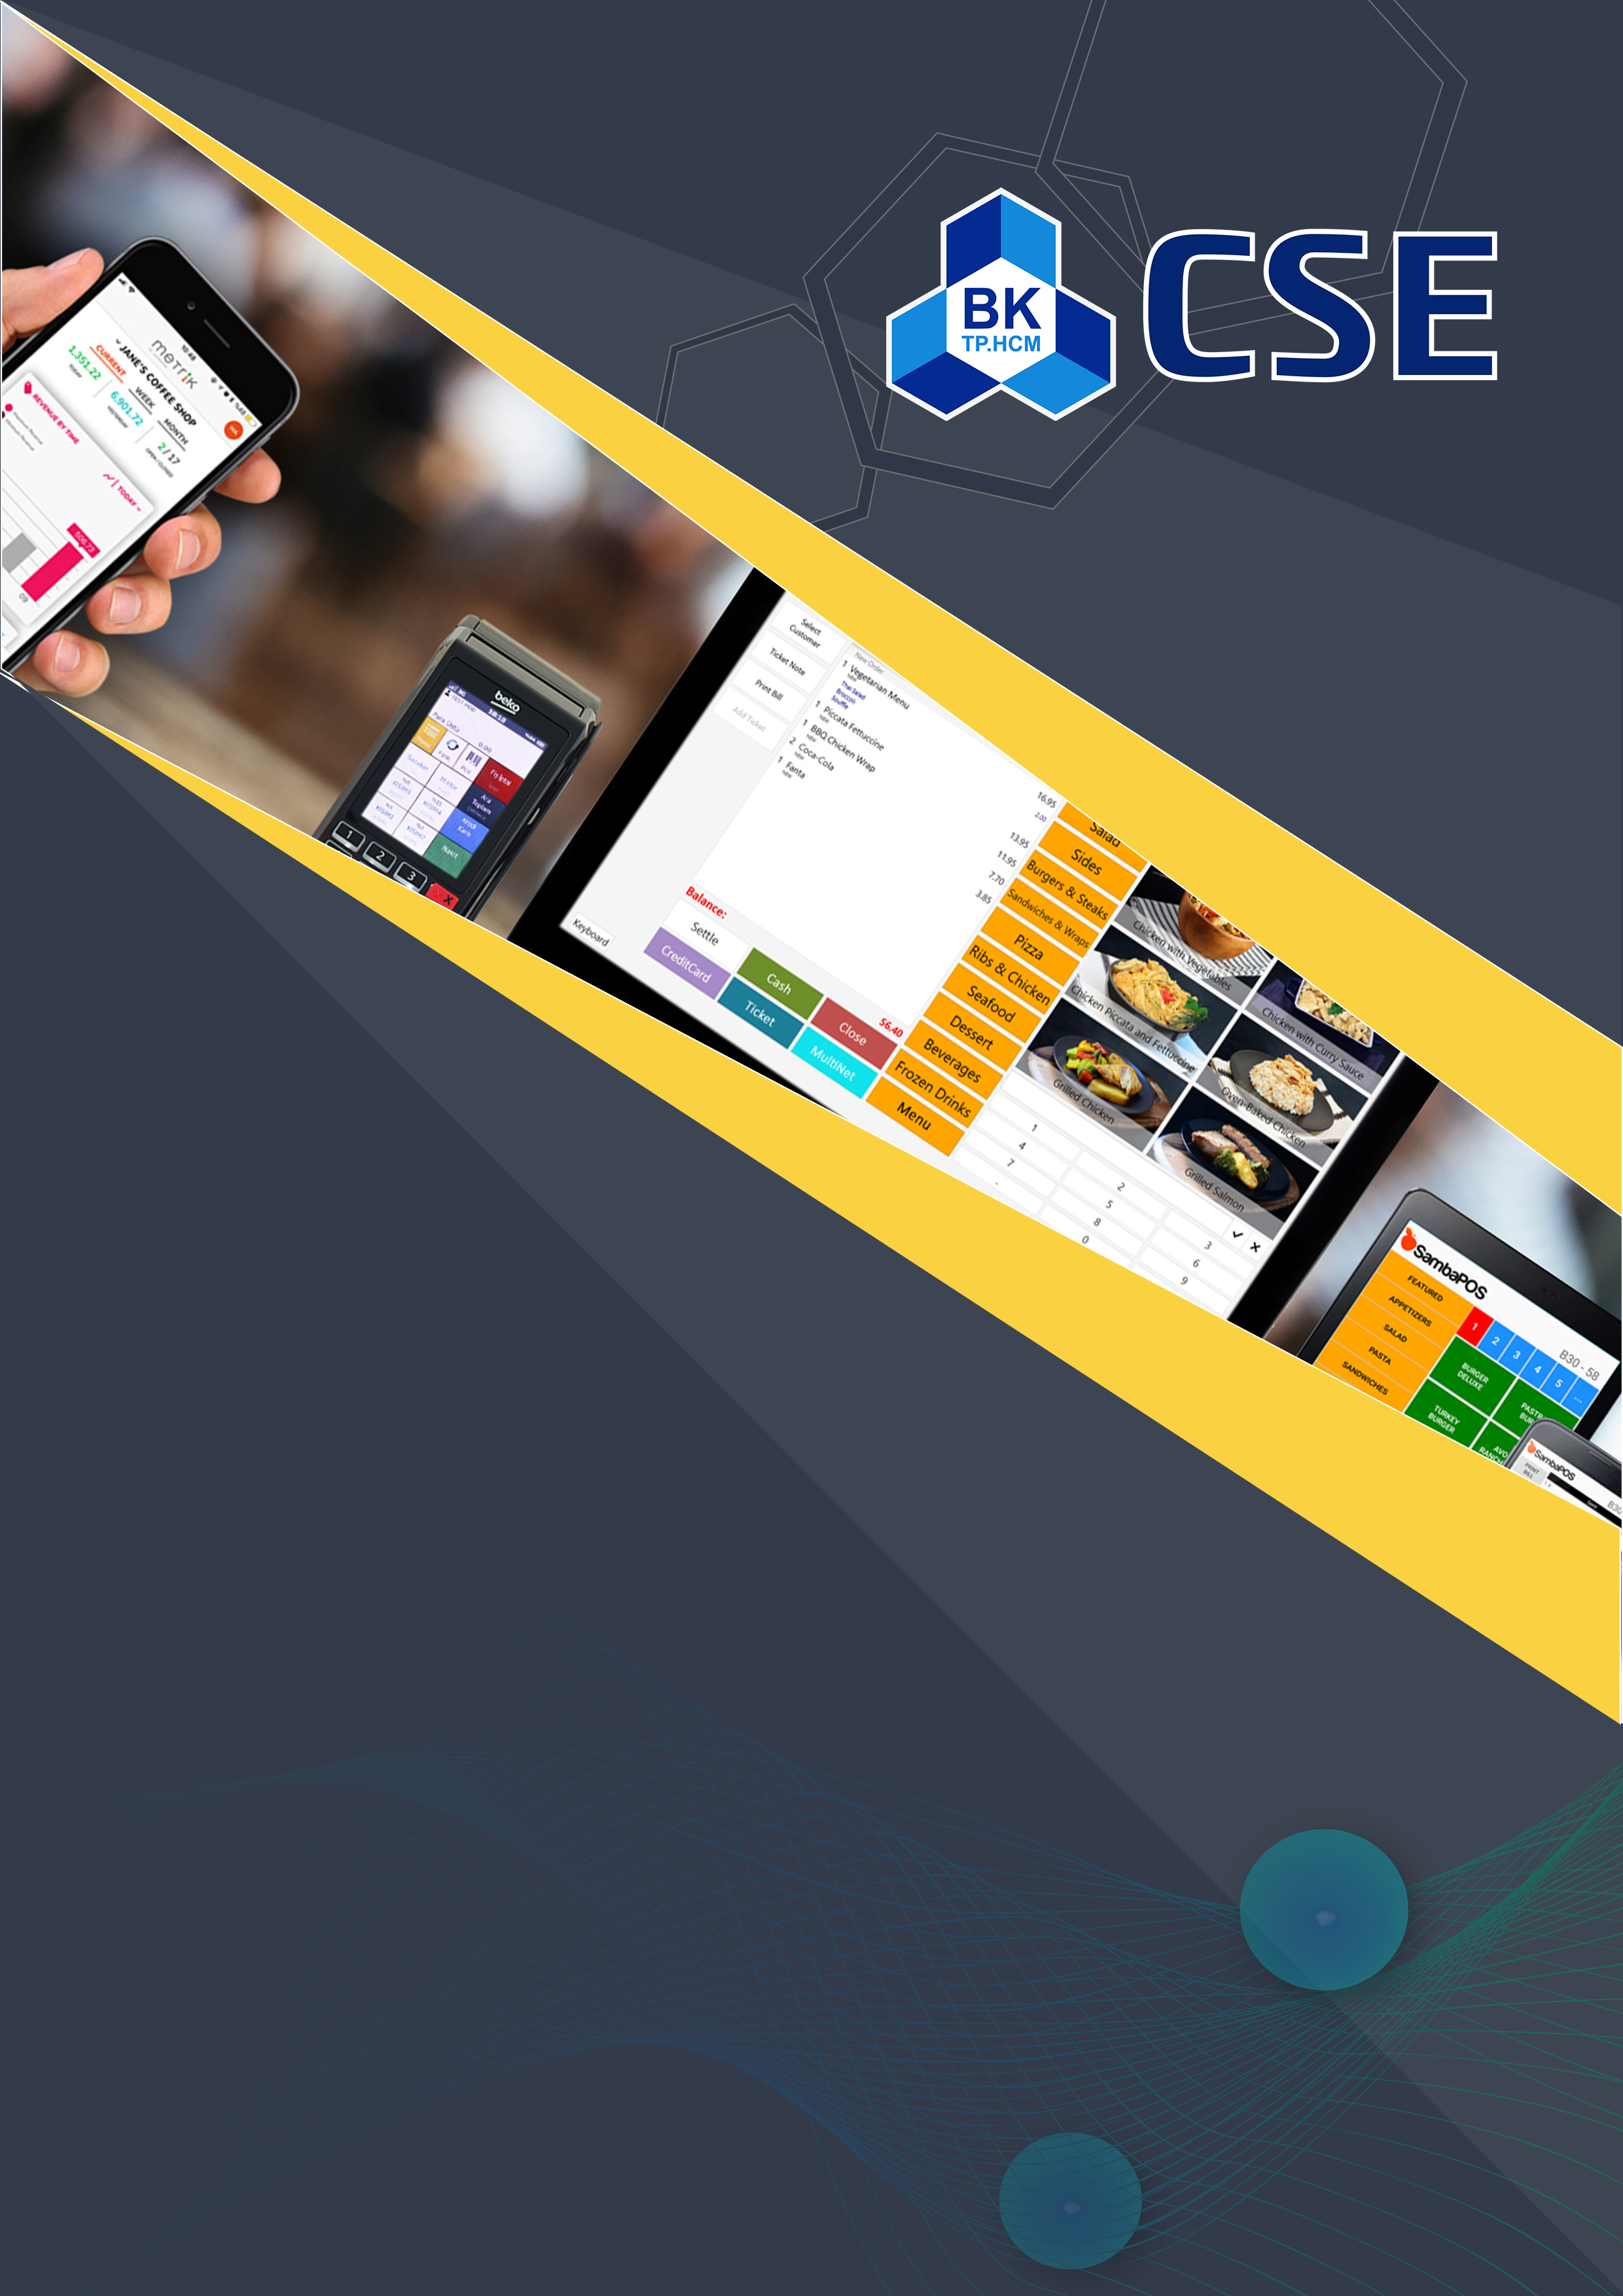
\includegraphics[width=220mm,scale=0.5]{Untitled-1}};
	
	
	\fontfamily{phv}\fontseries{b}\fontsize{16}{10}\selectfont
	
	
	
	\flushleft
	
	\color{white}
	\vspace{55mm}
	\fontfamily{lmss}\fontseries{b}\fontsize{17}{10}\selectfont
	SOFTWARE ENGINEERING \\[5mm]
	PROJECT REPORT \\
	
	
	\vspace{20mm}
	\color{white}
	\fontfamily{put}\fontseries{m}\fontsize{35}{10}\selectfont
	\textbf{Point-of-Sale} \\[8mm] System Design
	
	\normalsize
	\vspace{10mm}

	
	
	\vspace{\fill} 
	
	\flushleft
	\end{titlepage}

\newpage
\newgeometry{
	a4paper,
	left=24.1mm,
	right=24.1mm,
	top=35mm,
	bottom=35mm
	}

\newpage
\thispagestyle{empty}
\vspace*{\fill}

\newpage
\justifying
\pagenumbering{gobble}
\section*{This project was proudly done by...}

\begin{table}[H]
	\resizebox{\textwidth}{!}{%
		\begin{tabular}{|c|c|c|c|}
			\hline
			\rowcolor[HTML]{DAE8FC} 
			\textbf{No.} & \textbf{Student ID} & \textbf{Student's name} & \textbf{Email address}           \\ \hline
			1            & 1952669             & \begin{otherlanguage}{vietnamese}Vũ Hoàng Hải\end{otherlanguage}            & hai.vu.tharios19@hcmut.edu.vn     \\ \hline
			2            & 1952088             & \begin{otherlanguage}{vietnamese}Lê Nguyễn Tân Lộc\end{otherlanguage}       & loc.lenguyentan@hcmut.edu.vn      \\ \hline
			3            & 1952536             & \begin{otherlanguage}{vietnamese}Nguyễn Lê Thảo Vy\end{otherlanguage}       & vy.nguyen8956@hcmut.edu.vn        \\ \hline
			4            & 1952937             & \begin{otherlanguage}{vietnamese}Nguyễn Văn Quang\end{otherlanguage}        & quang.nguyen.0310@hcmut.edu.vn    \\ \hline
			5            & 1952785             & \begin{otherlanguage}{vietnamese}Nguyễn Lý Đăng Khoa\end{otherlanguage}    & khoa.nguyen.bk\_2019@hcmut.edu.vn \\ \hline
		\end{tabular}%
	}
\end{table}

\newpage
\section*{FOREWORDS}
\setstretch{1.3}

The following project is both a documentation and application on a basic point-of-sale terminal that is usually operated on restaurant businesses. It describes the focal point of a point-of-sale system that enables non-direct contact between clerks and customers, using Web technology and QR code,  that is responsive enough to implement the current business flow below.

\begin{figure}[H]
	\centering
	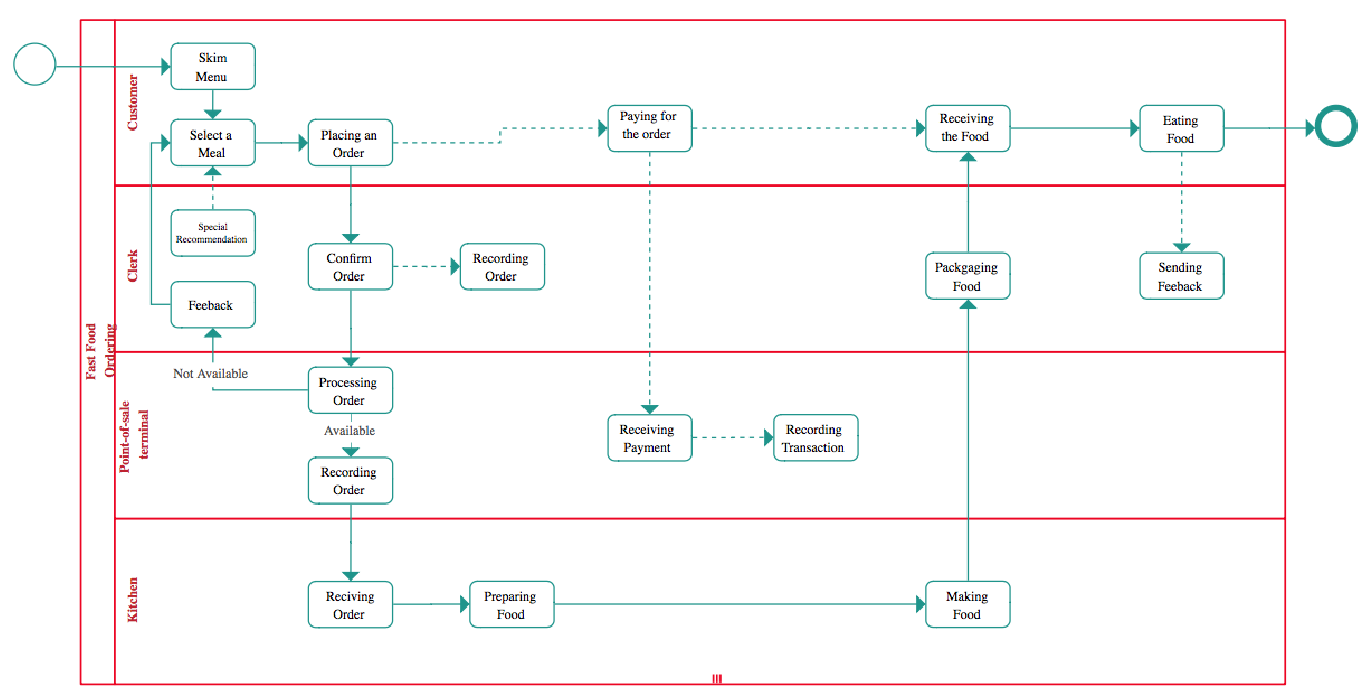
\includegraphics[width=16cm]{Screenshot 2022-02-17 144050.png}
	\caption{A universal restaurant point-of-sale system.}
\end{figure}

The proposed system in this project must be accessible from a mobile device, a tablet device or a normal computer, capable of error-free high workload and adaptive to future extensions.


\vspace{5mm}
This document is divided into multiple parts that will be progressively stated through the elicitation. Mainly, it will discuss requirement elicitation,  system modelling, architecture design and two sprints implementation of the system.


\newpage
\justifying
\pagenumbering{arabic}
\setcounter{page}{1}
\bluechaperNONUM
\tableofcontents
\normalsize
\standardchapterstyle

\bluechaperstyle
\newpage \setstretch{1.15}
\section*{Requirement elicitation}
\addcontentsline{toc}{section}{\protect\numberline{A}Requirement elicitation}%
\setstretch{1.3}

This section illustrates the contextual foundation idea of the entire project and give insights on how each functional block of the proposed system works. As such, the objectives of the system, the enriching scope, the sub-requirements for each interactive component are discussed in-depth.

\titlelabel{\thetitle.\quad}
\section{Project briefing}
\subsection{Context}
This project is targeted to be a web-based point-of-service (POS) system that empowers restaurants administrative with class management tools in order to operate their business efficiently. Apart from the regular dine-in service mode, this system also incorporates Internet-based and QR-code-enabled applications to address the difficulties occurred during the COVID-19 pandemic. It facilitates simplified, straight-forward and contact-less interactions between restaurant customers and staffs, e.g. food ordering, servicing, and payment in any convenience. The application also supports automation of various internal restaurant management tasks, such as order recording, order status managing, transaction recording, etc.

\begin{figure}[H]
	\centering
	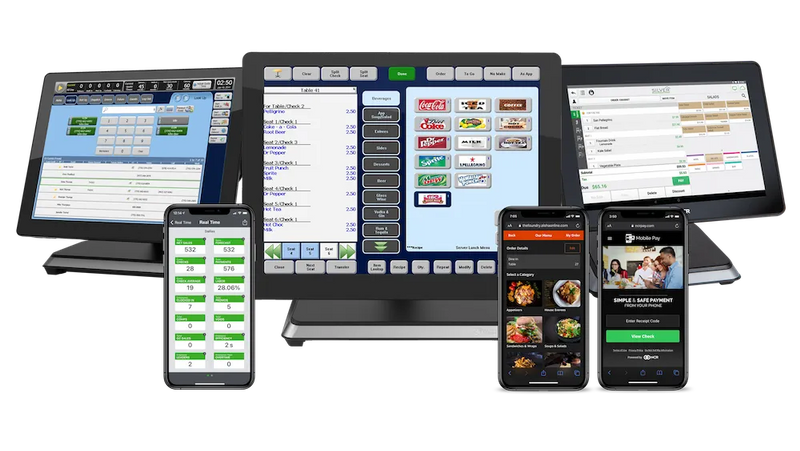
\includegraphics[width=16cm]{61017fc978f5606b7f0ee2de_aloha-essentials-and-silver-no-orderpay-p-800.png}
	\caption{A universal restaurant point-of-sale system.}
	\label{fig:adafruitdashboard}
\end{figure}

\subsection{Stakeholders}

The relevant stakeholders of this proposed system may include human resources such \textit{restaurant owner, managers}, and \textit{staff} (including clerks, chefs and janitors), and external consumerism, e.g. \textit{restaurant customers/clients}.

\subsection{Features}
The system consists of the following features that enable the complete functionality:

\begin{itemize}\setstretch{1.1}
	\item A \textit{menu screen} for displaying the restaurant's menu; customers can make their selections in this screen.
	\item A \textit{detail screen} for each food, which will provide pictures and/or related information of a specific food.
	\item A \textit{cart} that visually display customer’s selected food; this screen allows customers to re-check, edit and place their orders.
	\item  A \textit{payment screen} that offers different payments options.
	\item An \textit{order processing screen} that will be displayed while the food being made; this screen contains status of customer’s pending order.
	\item A \textit{feedback screen} to receive customers’ feedback on qualities of the restaurant’s food and services.
\end{itemize}

\subsection{Scopes}

The central objective of this project is to propose a web-based solution
for restaurant owners, to help them maintain the normal operation of their business, while limiting physical / direct interactions between restaurant customers and staff as much as possible. To illiterate in clearer details, the in and out scopes are as follows: 

\subsubsection{In scope}
\begin{itemize}\setstretch{1}
	\item A responsive website with attractive UI, categorization, filter and search functionality.
	\item A back-end system to provide support for multiple restaurants, with the
	ability of handling approximately 300 transactions per day.
	\item An online database that supports inventory management.
\end{itemize}

\subsubsection{Out of scope}
\begin{itemize}\setstretch{1}
	\item Interactive platform to facilitate contactless interactions between
	restaurant staff.
	\item Restaurant staff management system.
	\item Delivery management system.
	\item Payment processing system.
\end{itemize}

\section{Requirements and use-casing}
The following section describes the all functional and non-functional requirements in context of the desired system. A use case diagram is also presented to cohesively illustrate the interactions of the said system.

\subsection{Functional requirements}

\begin{enumerate}[label=\alph*., font=\itshape]
	\item \textbf{Search and filter menu}:
	\begin{itemize}
		\item The system shall display all available options that the restaurant provides by default.
		\item The menu screen is visible to all inusers.
		\item The system shall display detailed information of a selected item.
		\item The system shall display detailed food categorization to user when
		needed.
		\item The system shall enable user to enter search text to the search box.
		\item The system shall display all matching results based on the search text.
		\item The system shall enable user to apply one or more filter(s) to the search
		result.
		\item The system shall allow user to navigate between the search results.
		\item The system shall notify user when no matching result can be found.
	\end{itemize}

	\item \textbf{Account registration (log in/log out)}:
	\begin{itemize}
		\item The system shall require staff members logged in before performing any task. Customers with affiliated membership programs can log in to enjoy exclusive benefits.
		\item The system shall keep record of all activities of each account.
		\item The system shall grant different privileges for each specific type of user: customer-type user can place order and have no access to internal information; clerk-type user / kitchen-type user / manager-type user will have permission to edit their position-related information on the system.
		\item The system shall require customer-type user to enter his / her telephone number and a password in order to create an account.
		\item The system shall allow manager-type user to create new staff-type account(s).
		\item The system shall allow manager-type user to edit restaurant menu, modify	several types of inventory and view all internal data.
		\item The system shall allow clerk-type user and kitchen-type user to assign some specific statuses to pending order(s).
		\item The system shall enable kitchen-type user to modify cooking-related inventory, including ingredients, cooking supplies, kitchen utensils and appliances.
	\end{itemize}
	
	\item \textbf{Editorial menu}:
	\begin{itemize}
		\item The system shall only allow manager-type user to edit the menu.
		\item The system shall allow manager-type user to add / remove item(s) in the menu.
		\item The system shall allow manager-type user to add / remove / edit related information of any item.
		\item The system shall support different types of tags to be assigned to items, such as \textit{"new"}, \textit{"hot"}, \textit{"sale"}, etc.
		\item Each item can have one or more tag(s) at a time.
	\end{itemize}

	\item \textbf{Update order status / update cooking progress}:
	\begin{itemize}
		\item Every order can have one status at any given time.
		\item The status of an order is visible to the customer who ordered it, the clerk who is in charge of it and the kitchen staff.
		\item The system shall allow clerk-type user to assign \textit{“received”} status for newly-submitted order(s); \textit{“not available”} in case of one or more item(s) in an order is unavailable; \textit{“confirmed”} for fully-available order(s) which can be forward to the kitchen and \textit{"completed"} for those that have been successfully finished.
		\item The system shall allow no change on order(s) marked as \textit{“completed”}.
		\item The system shall allow kitchen-type user to make some updates on their cooking process, by assigning \textit{“processing”} to orders that are being prepared and \textit{“ready”} to those that are ready to serve / packed.
	\end{itemize}
	
	\item \textbf{Manage inventory}:
	\begin{itemize}
		\item The system shall only allow staff-type user (manager-type and kitchen-type) to access inventory information.
		\item The system shall enable kitchen-type user to add / remove / change the quantity of cooking related items (ingredients; cooking supplies; kitchen utensils and appliances).
		\item The system shall allow manager-type user to add / remove / change quantity of items that are not taken care by kitchen-type user (service supplies; packing materials; maintenance, repairs and operating goods).
		\item The system shall notify staff-type user (manager-type and kitchen-type) if the amount of any item in their charge goes below 10.
		\item The system shall record any change made on inventory information, including who made the change, its timestamp and the change description.
	\end{itemize}
	
	\item \textbf{Make an order}:
	\begin{itemize}
		\item The system shall allow customer-type user to select between eat-in, take-away or delivery.
		\item In case delivery is selected, customer shall be directed to a third party delivery platform.
		\item The system shall allow customer-type user to add minimum 1 and maximum 30 separate items to his / her cart.
		\item The system shall allow customer-type user to edit his / her cart.
		\item The system shall calculate and display the total price of the order.
		\item The system shall allow customer-type user to place his / her order.
		\item The system shall notify online clerk-type user when a new order is placed.
		\item The system shall notify kitchen-type user when a new order is forwarded to be cooked.
		\item The system shall notify customer-type user once his / her order is marked as \textit{“completed”}, display the invoice and ask for his / her feedback.
	\end{itemize}

	\item \textbf{Make payment}:
	\begin{itemize}
		\item The system shall allow customer-type user to choose one from a list of online payment methods to proceed.
		\item The system shall forward customer-type user to his /her selected payment platform.
		\item The system shall check whether the transaction is made successfully and notify clerk-type user.
	\end{itemize}

	\item \textbf{Give / display feedback}:
	\begin{itemize}
		\item The system shall allow customer-type user to give feedback on food and service quality.
		\item The system shall display the feedback of every item.
		\item The system shall enable user to filter the feedback of each item by date and rating.
		\item The system shall allow customer-type user to edit his / her feedback.
	\end{itemize}

	\item \textbf{View and manage business data}:
	\begin{itemize}
		\item The system shall keep record of every completed invoice.
		\item The system shall allow manager-type user to access business data and statistics.
		\item The system shall allow manager-type user to filter the restaurant business	data and sort them as needed.
		\item The system shall display an overall summary for statistics for manager-type user if needed.
	\end{itemize}
\end{enumerate}

\subsection{Non-functional requirements}

\begin{itemize}
	\item The server is kept to be always online to ensure synchronization. Active hours includes from 6am to 10pm, customers can use all functions during the period. After those hours, customer can make reservation in advance.
	
	\item The website should have a consistent scale, design, look, and responsiveness on different devices and offers easy to use and have instructional videos for customers.
	
	\item Maintenance to the system is performed every 4 months. Each periodic and progressive system upgrades should not last more than 30 minutes and happen in the hour that has the least customer traffic to avert unintended congestion.
	
	\item UI/UX should be modern and user-friendly, system respond time to users is allowed no more than 3 seconds.
	
	\item System must be decentralized, users have their unique permission to access different data. Customer databases must be encrypted end-to-end.
		
	\item The system e-invoice must follow the legal government laws of creating and using online invoices, as well as cyber security law. (\textit{Circular No. 32/2011/TT-BTC, dating March 14th, 2011, and decree 119/2018/ND-CP dating September 12th, 2018})

\end{itemize}

\newpage
\subsection{System use-case diagram}
Figure \ref{fig:systemusecase} shows the use-case diagram representation for the entire system.

\begin{figure}[H]
	\centering
	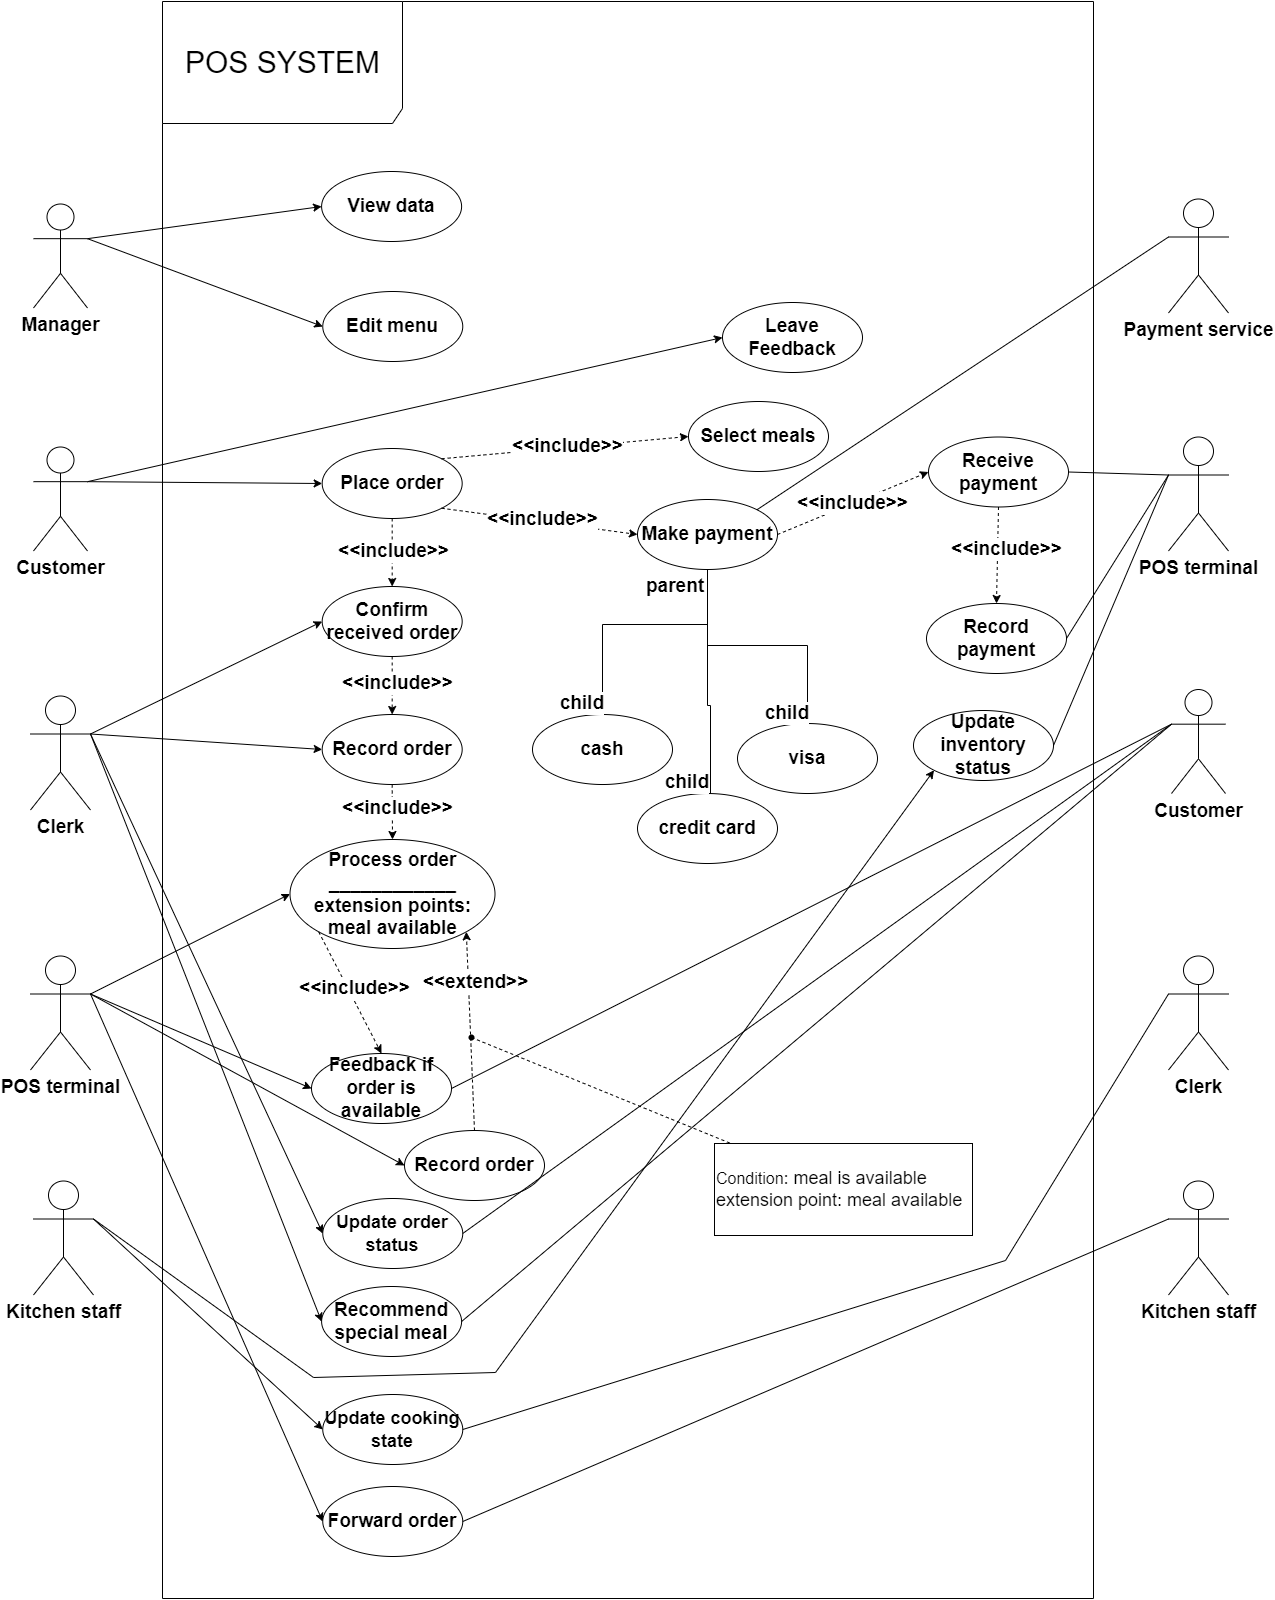
\includegraphics[width=15.5cm]{259243473_617353449353167_471014773977634987_n.png}
	\caption{Overall system use-case of a proposed restaurant point-of-sale.}
	\label{fig:systemusecase}
\end{figure}

\newpage
\section{Food ordering use-case example}
Figure \ref{fig:foodusecase} shows an in-depth use-case diagram of a \textit{food ordering} system feature.

\begin{figure}[H]
	\centering
	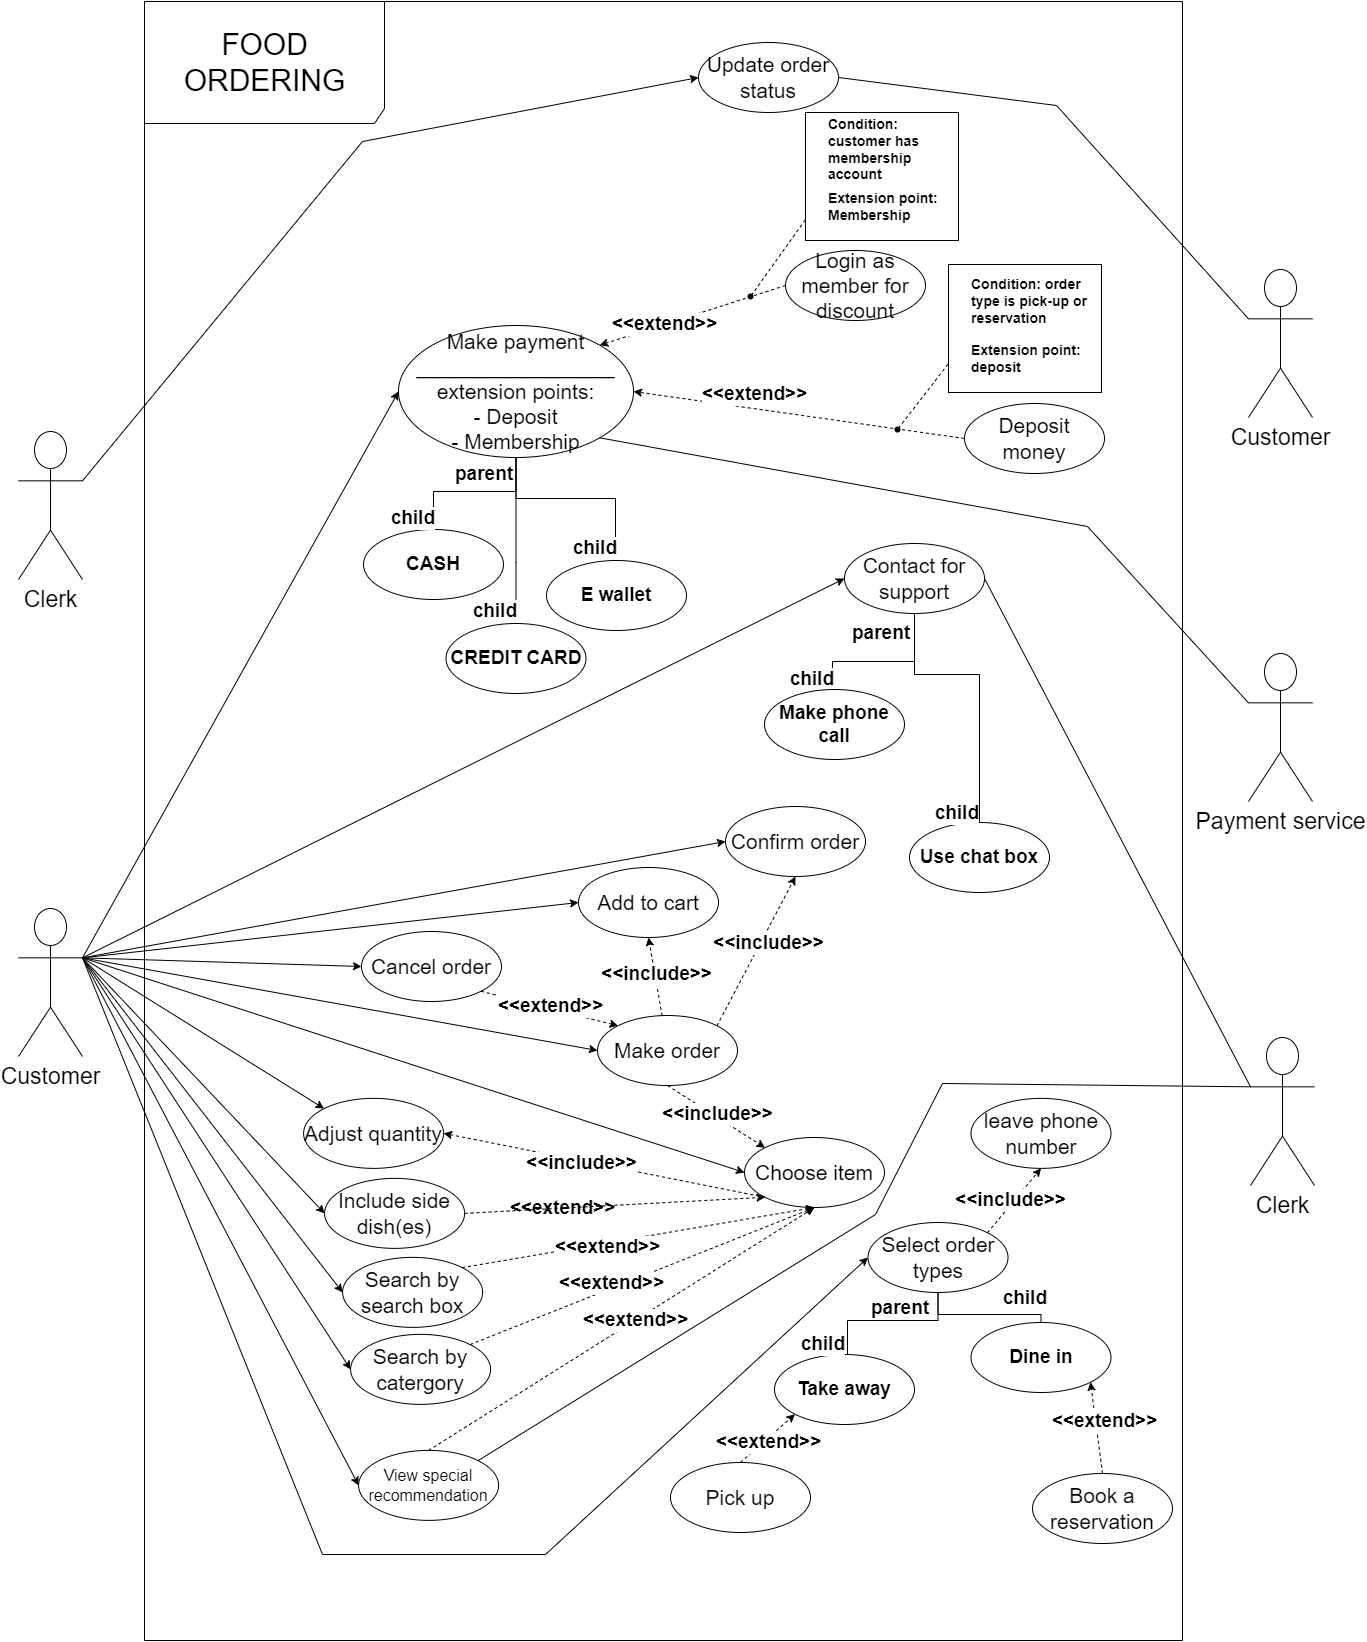
\includegraphics[width=15.5cm]{272520954_703266950872464_5753385862413650595_n.png}
	\caption{Food ordering use-case of a proposed restaurant POS feature.}
	\label{fig:foodusecase}
\end{figure}

In order to dissect this diagram in a friendly manner, the following table \ref{tab:foodorder} will describe the use-case in details:

\begingroup
\renewcommand\arraystretch{1.5}
\begin{longtable}{>{\centering\bfseries\columncolor[HTML]{DAE8FC}{}}m{3.25cm} >{\arraybackslash}m{12cm}}
		\hline
		Use-case \\ description & A feature of POS system that aims to help customer get access to all available services of the restaurant including make food order with different order types (dine-in, take-away), select meals via multiple searching methods (catergory searching, search by name) or view special recommendations of the restaurant. To ask for assistance, customer may contact the clerk via chat box or direct phone call. Further more, the feature supports multiple payment methods apart from cash such as credit card, E wallet. \\
		\hline
		Primary actors & Customer and Clerk. \\
		\hline
		Secondary actors & 
		Customer, Clerk and Payment service. \\
		\hline
		Pre-condition & Customer must have access to the web page by scanning provided QR code or through Internet hyperlink. \\
		\hline
		Post-condition & The customer payment is verified and they have had their food served. \\
		\hline
		Main flow & \begin{enumerate}[leftmargin=*]\setlength\itemsep{-0.1cm}
			\item Customers access the webpage by scanning the QR code or by Internet hyperlink.
			\item Customers choose to dine-in without booking reservation in advance.
			\item A menu pops up with different combinations of meals and drinks.
			\item Customers select one of the displayed choice or search for a specific one via a search box or they can view some special recommendations from the restaurant in a window.
			\item After choosing the meals, customers add them to cart.
			\item Customers confirm their order.
			\item Customers pay for their order via credit card, e-wallet, or direct cash.
			\item Customer leaves phone number.
			\item Once food is ready to serve, the system will inform the customer by their phone number SMS or notification.
		\end{enumerate} \\
			\hline
		Alternative flow & \begin{enumerate}[leftmargin=*]\setlength\itemsep{-0.1cm}
			\item Customers access the webpage by scanning the QR code or by Internet hyperlink.
			\item Customer books a table reservation in the restaurant.
			\item A menu pops up with different combos of meals and drinks.
			\item Customer selects one of those displayed, search for a specific one via a search box or they can view some special recommendations from the restaurant.
			\item After choosing the meals, customer adds them to cart.
			\item Customer confirms the order.
			\item Customer deposits money for the table reservation.
			\item Customer leaves phone number.
			\item The system will send SMS or notification to customer 15 minutes before the booked time.
		\end{enumerate} \\
		\hline
		\caption{Food ordering glossary}
		\label{tab:foodorder}
\end{longtable}
\endgroup

\newpage
\section*{System modeling}
\addcontentsline{toc}{section}{\protect\numberline{B}System modeling}%
\setstretch{1.3}

This section will perform laid-out diagrams to capture the major  functional requirements of the
desired restaurant POS system. It is divided into three caconicals of an activity diagram, a sequence diagram and a class diagram.

\setcounter{section}{0}
\section{Activity diagram} 

\textbf{Figure \ref{fig:actdiag}} shows an activity diagram of a restaurant POS that condenses the major functional requirements of the entire system.


\section{Sequence diagram} 

\textbf{Figure \ref{fig:seqdiag2}} shows a sequence diagram of a restaurant POS that has object interactions arranged in predefined time sequence.

\section{Class diagram} 

\textbf{Figure \ref{fig:classdiag}} shows a class diagram of a restaurant POS. This depicts the structure of the system by showing the system's classes, their attributes, operations (or methods), and the relationships among objects declared in \textbf{Section A}.


\begin{sidewaysfigure}
	\centering
	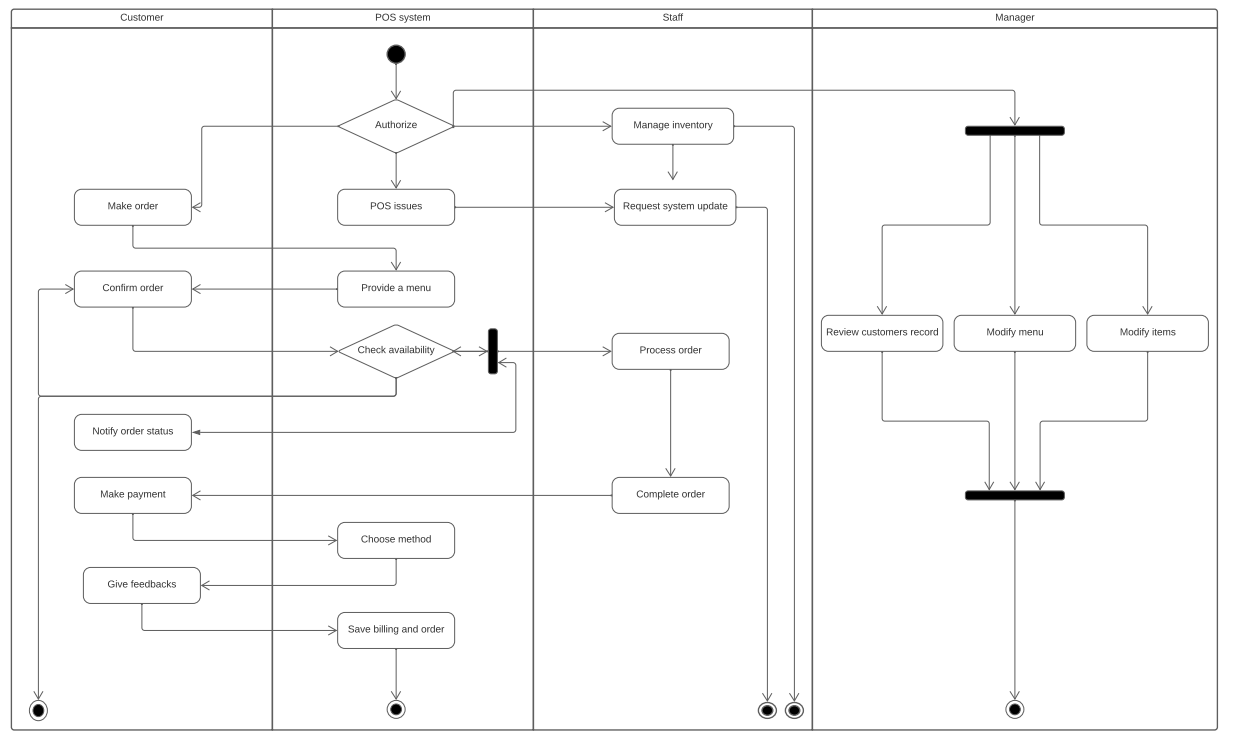
\includegraphics[width=23cm]{Screenshot 2022-03-05 180519.png}
	\caption{Activity diagram of a restaurant POS.}
	\label{fig:actdiag}
\end{sidewaysfigure}

\begin{figure}
	\centering
	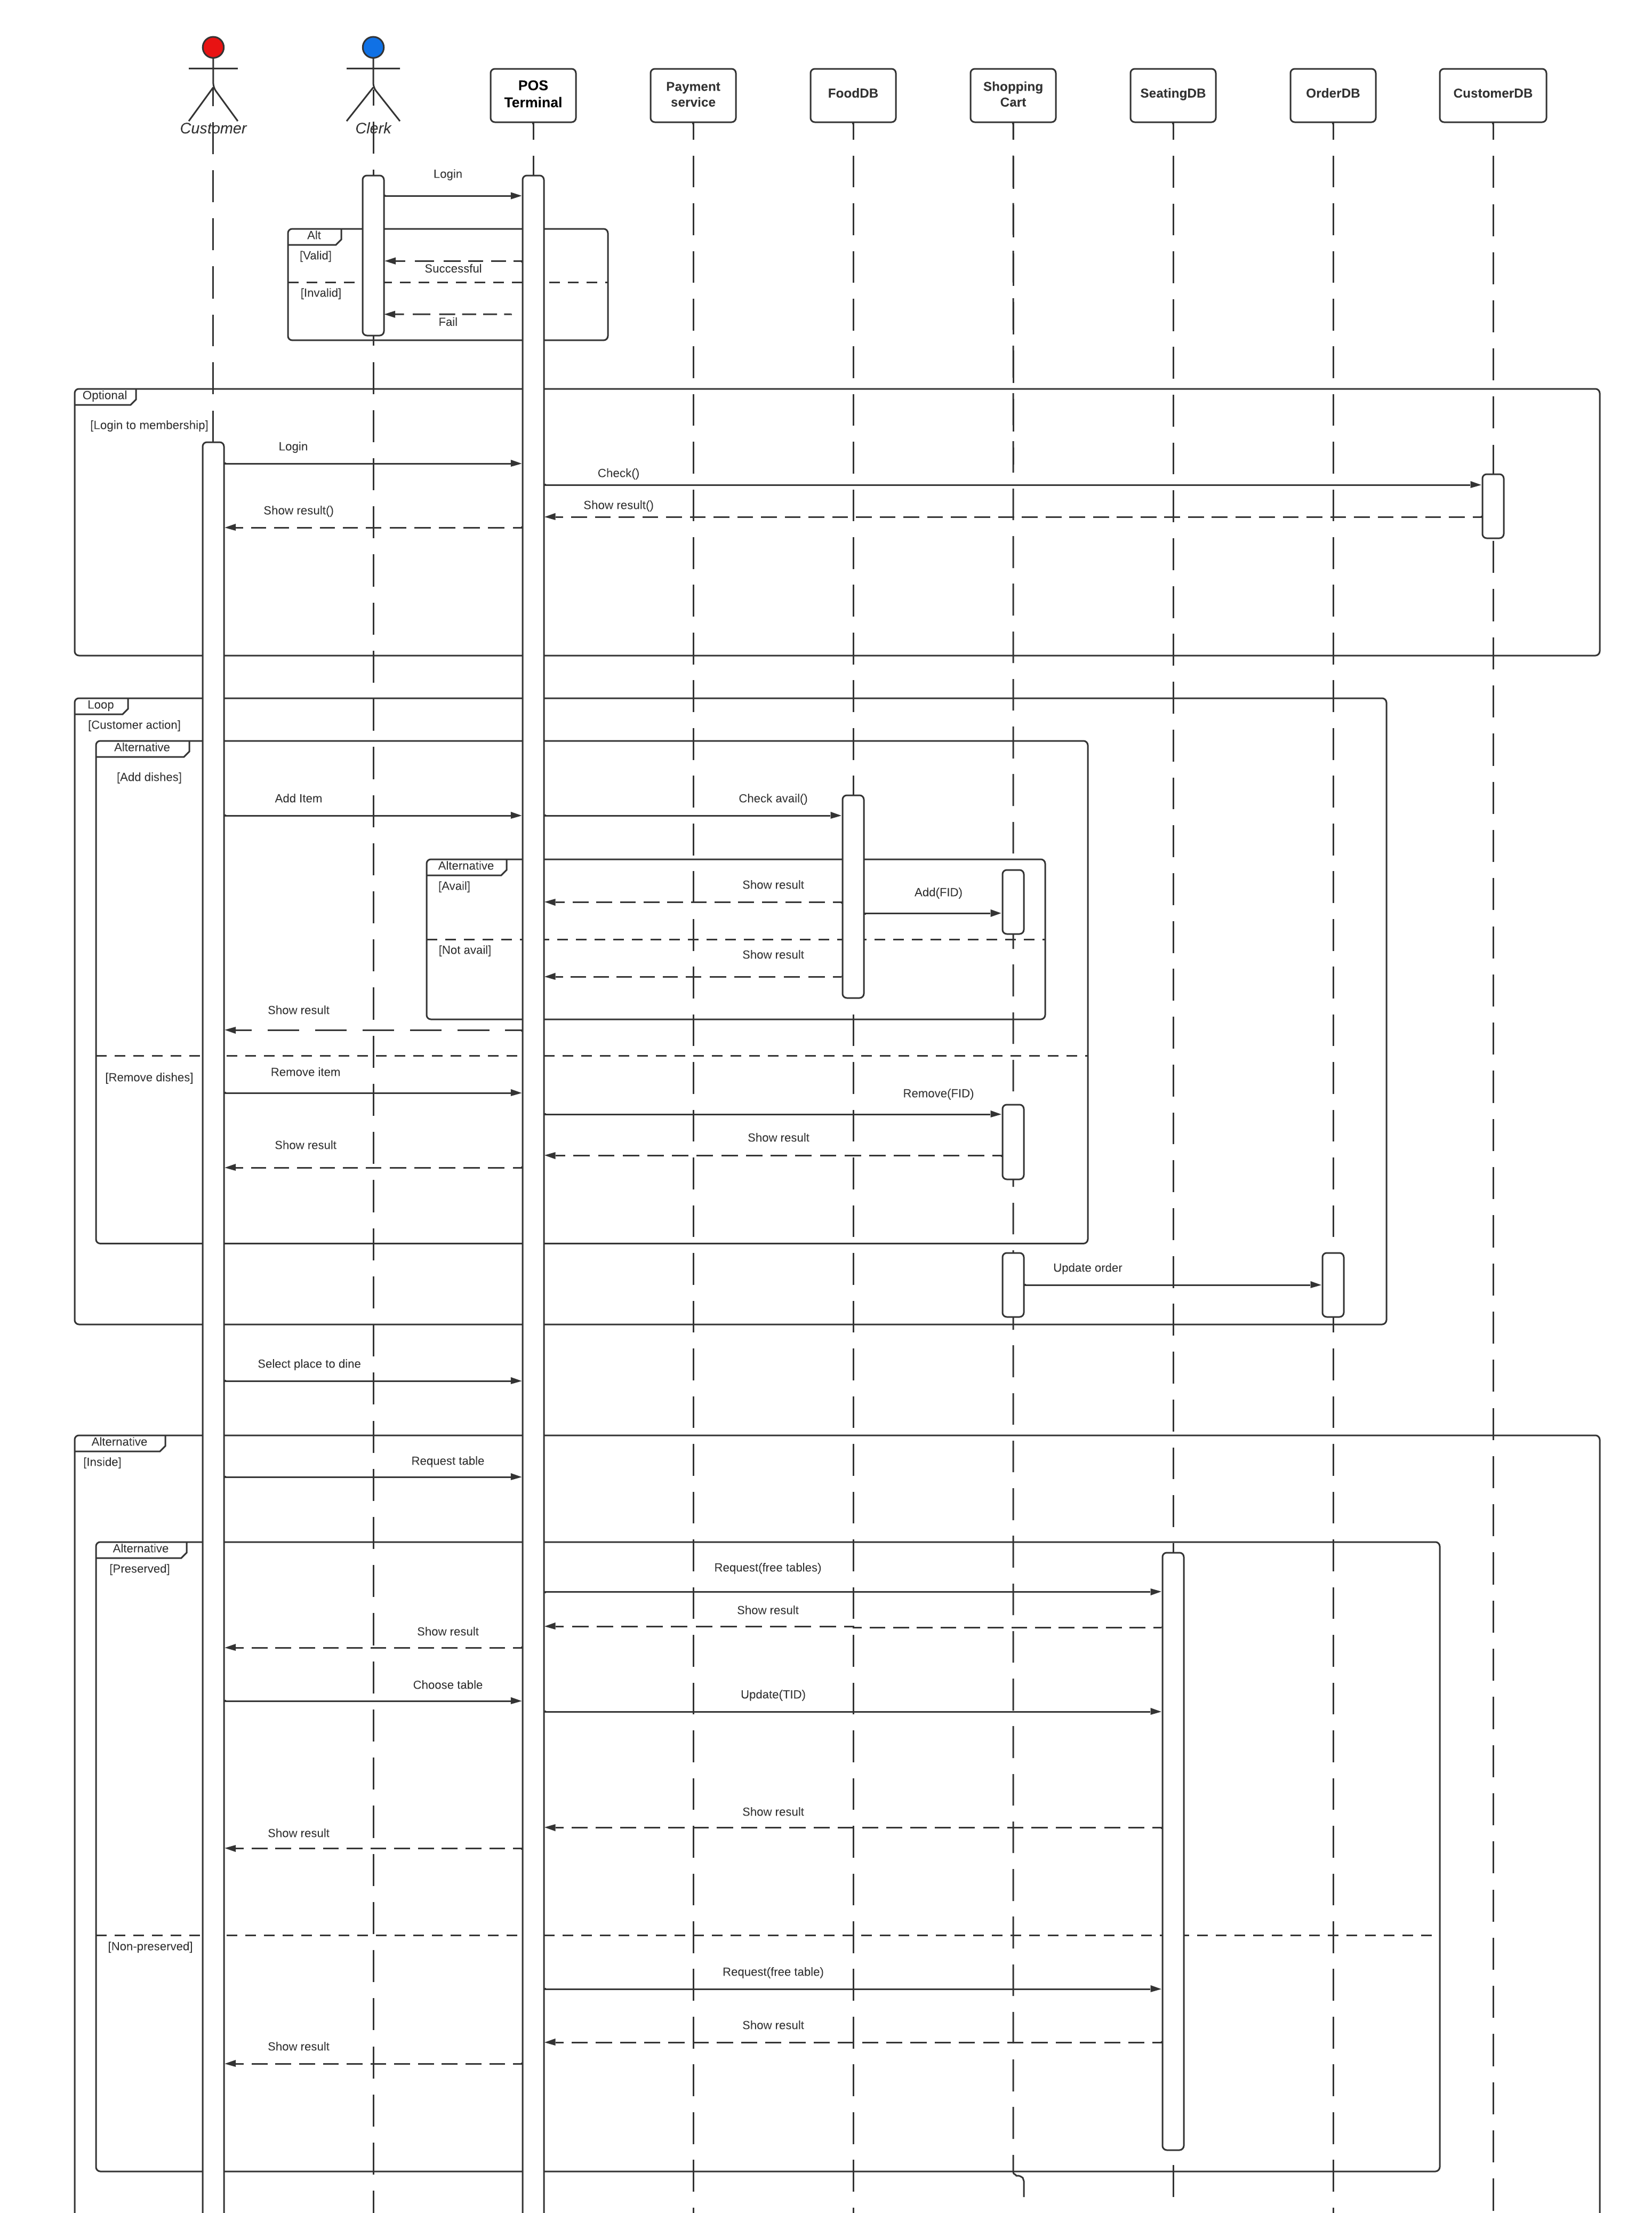
\includegraphics[width=16.5cm]{Screenshot 2022-03-05 182607.png}
	\label{fig:seqdiag1}
\end{figure}
\begin{figure}
	\centering
	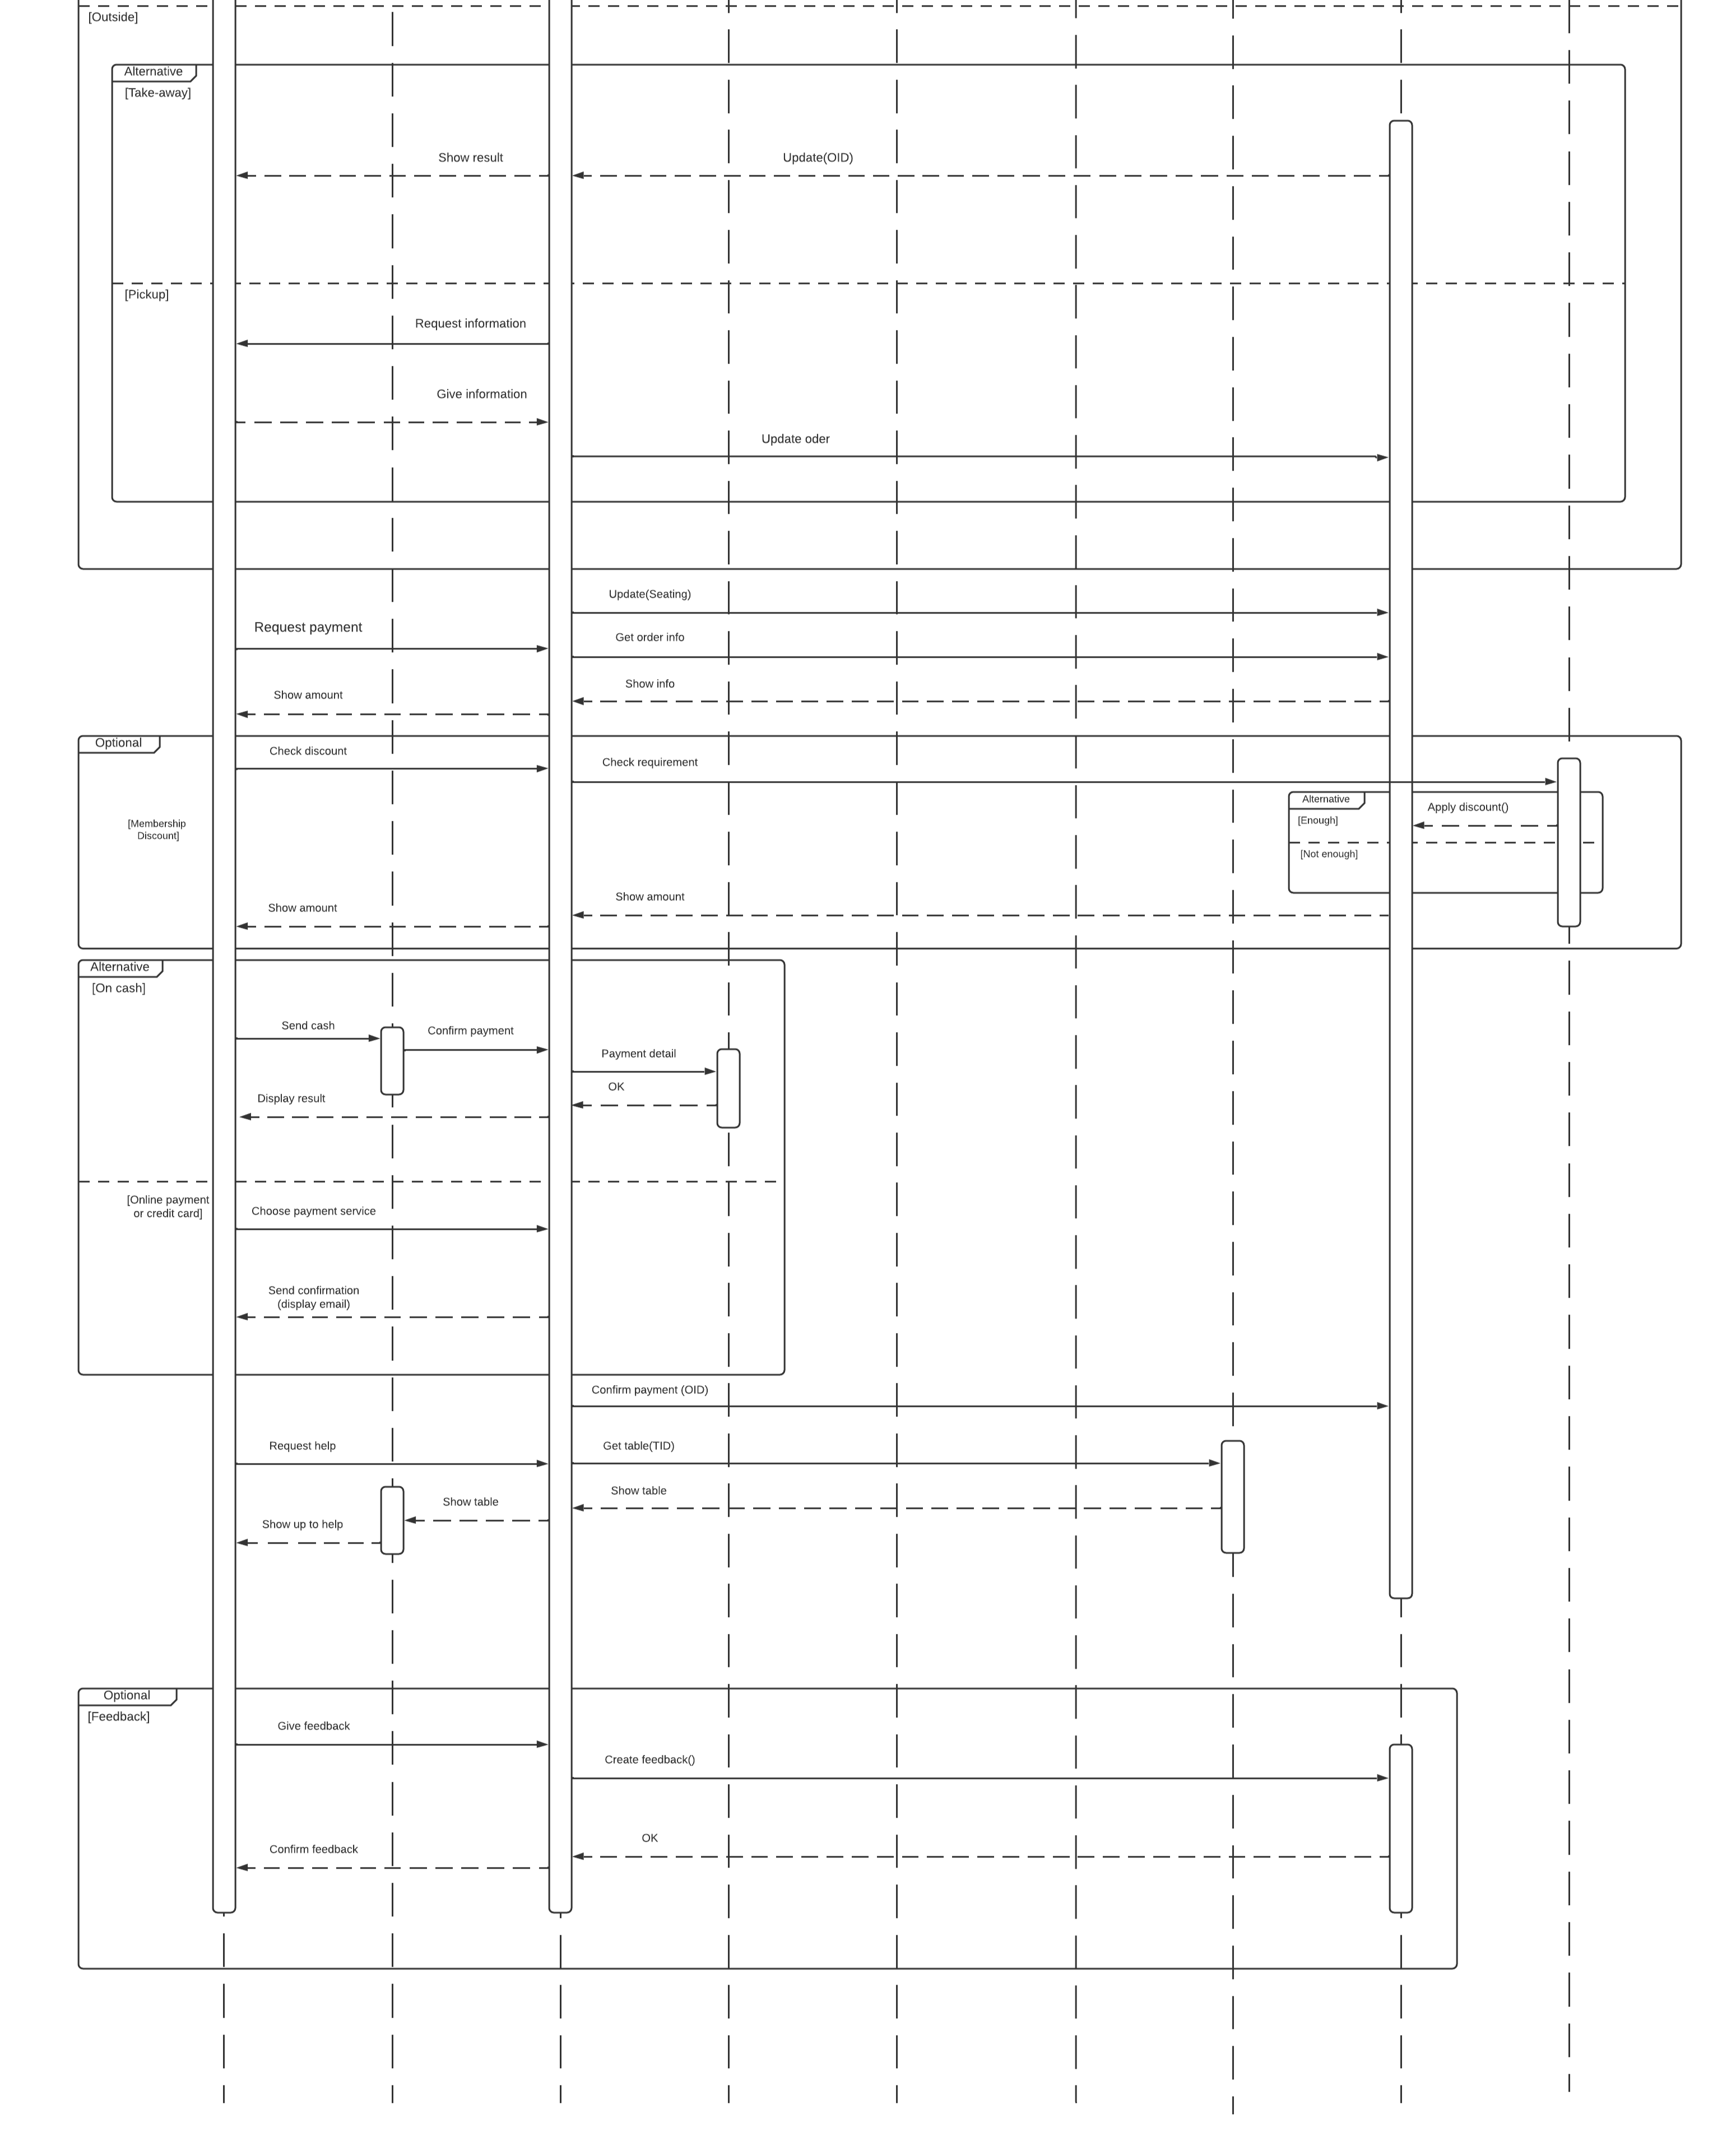
\includegraphics[width=16.5cm]{image.png}
	\caption{Sequence diagram of a restaurant POS.}
	\label{fig:seqdiag2}
\end{figure}

\begin{sidewaysfigure}
	\centering
	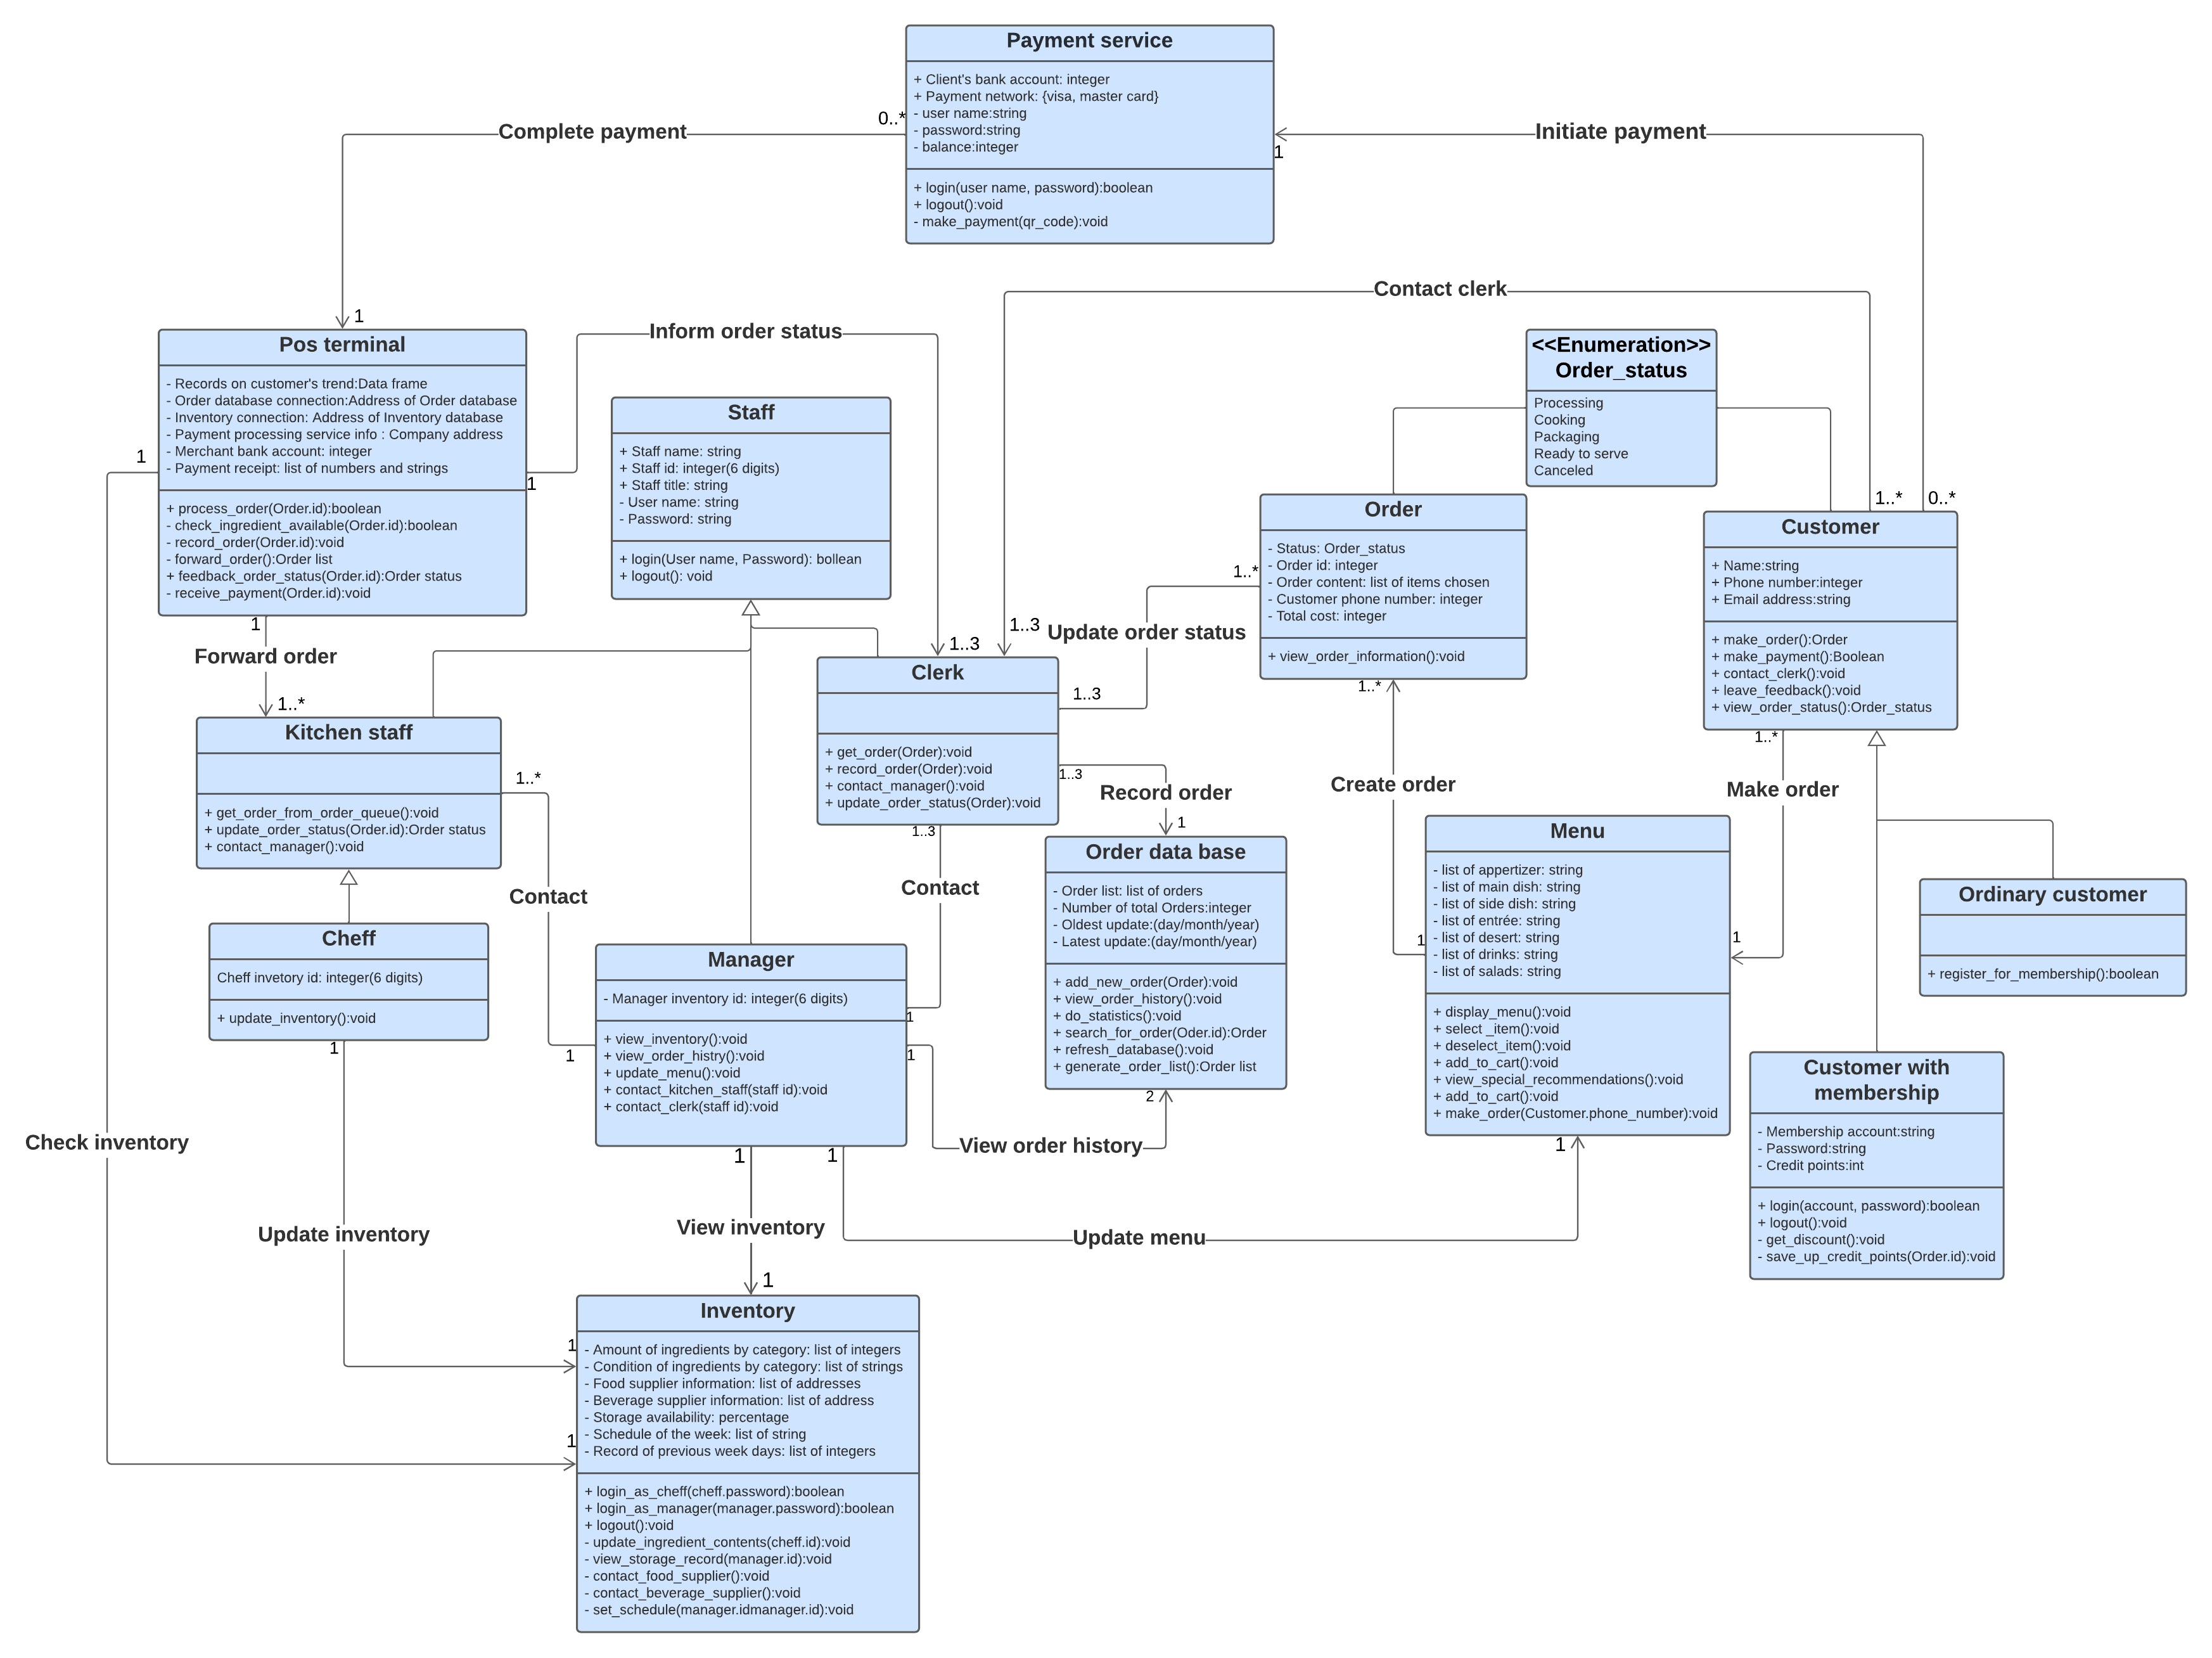
\includegraphics[width=23cm]{image (2).png}
	\caption{Class diagram of a restaurant POS.}
	\label{fig:classdiag}
\end{sidewaysfigure}

\newpage
\section*{System architecture}
\addcontentsline{toc}{section}{\protect\numberline{C}System architecture}%
\setstretch{1.3}
	
A fundamental approach to visualize the structural integrity of the entire restaurant point-of-sale system presented in this project is via a cohesive blueprint of the overall architecture. In this section, all of the foundational components of the application are described in detail, with reasoning of choice and facilitation. They are then described further in implementation diagrams to better illustrate the said functional requirements in \textbf{Section A}. 

\setcounter{section}{0}
\section{Cloud-native architecture pattern} 

There are numerous architectural patterns that capture the design structures of various systems and elements of software so that they can be reused. For this project's system, to fully utilize the power of cloud-based ordering point-of-sale, using \textit{application programming interfaces (APIs)} instead of a fixed model, a much more advanced version of \textit{Model-View-Controller (MVC)} pattern is needed.

\subsection{Architecture foundation}

\textit{Cloud-native architecture} is a suitable upgrade for MVC. It allows dynamic and agile application development techniques that take a modular approach (API with user-interfaces and services) to building, running, and updating software through a suite of cloud-based microservices and containerization with agility and dynamism versus a monolithic application infrastructure.

\vspace{5mm}
The entire architecture is depicted as a triangular representation in \textbf{Figure \ref{fig:archdiag}}. This is a close-knit relationship (represented by outer connecting edges) between sub-API gateways: \textbf{delegate} for the major operative branches of the restaurant system, \textbf{online} for activities done over the Internet, and \textbf{management} for internal affairs. Each of these has their own separate sets of user-interfaces, services and database buffers to handle tasks independently. Communication is established to the central core API to perform requests made from the sub-APIs and to keep synchronization between sub-API databases and the central database.

\subsection{Integration and security advantages}

It can be seen from the network the central database can only be accessed via the core API. This proposed architecture provides an efficient security layer that separates the master storage from 

\begin{sidewaysfigure}
	\centering
	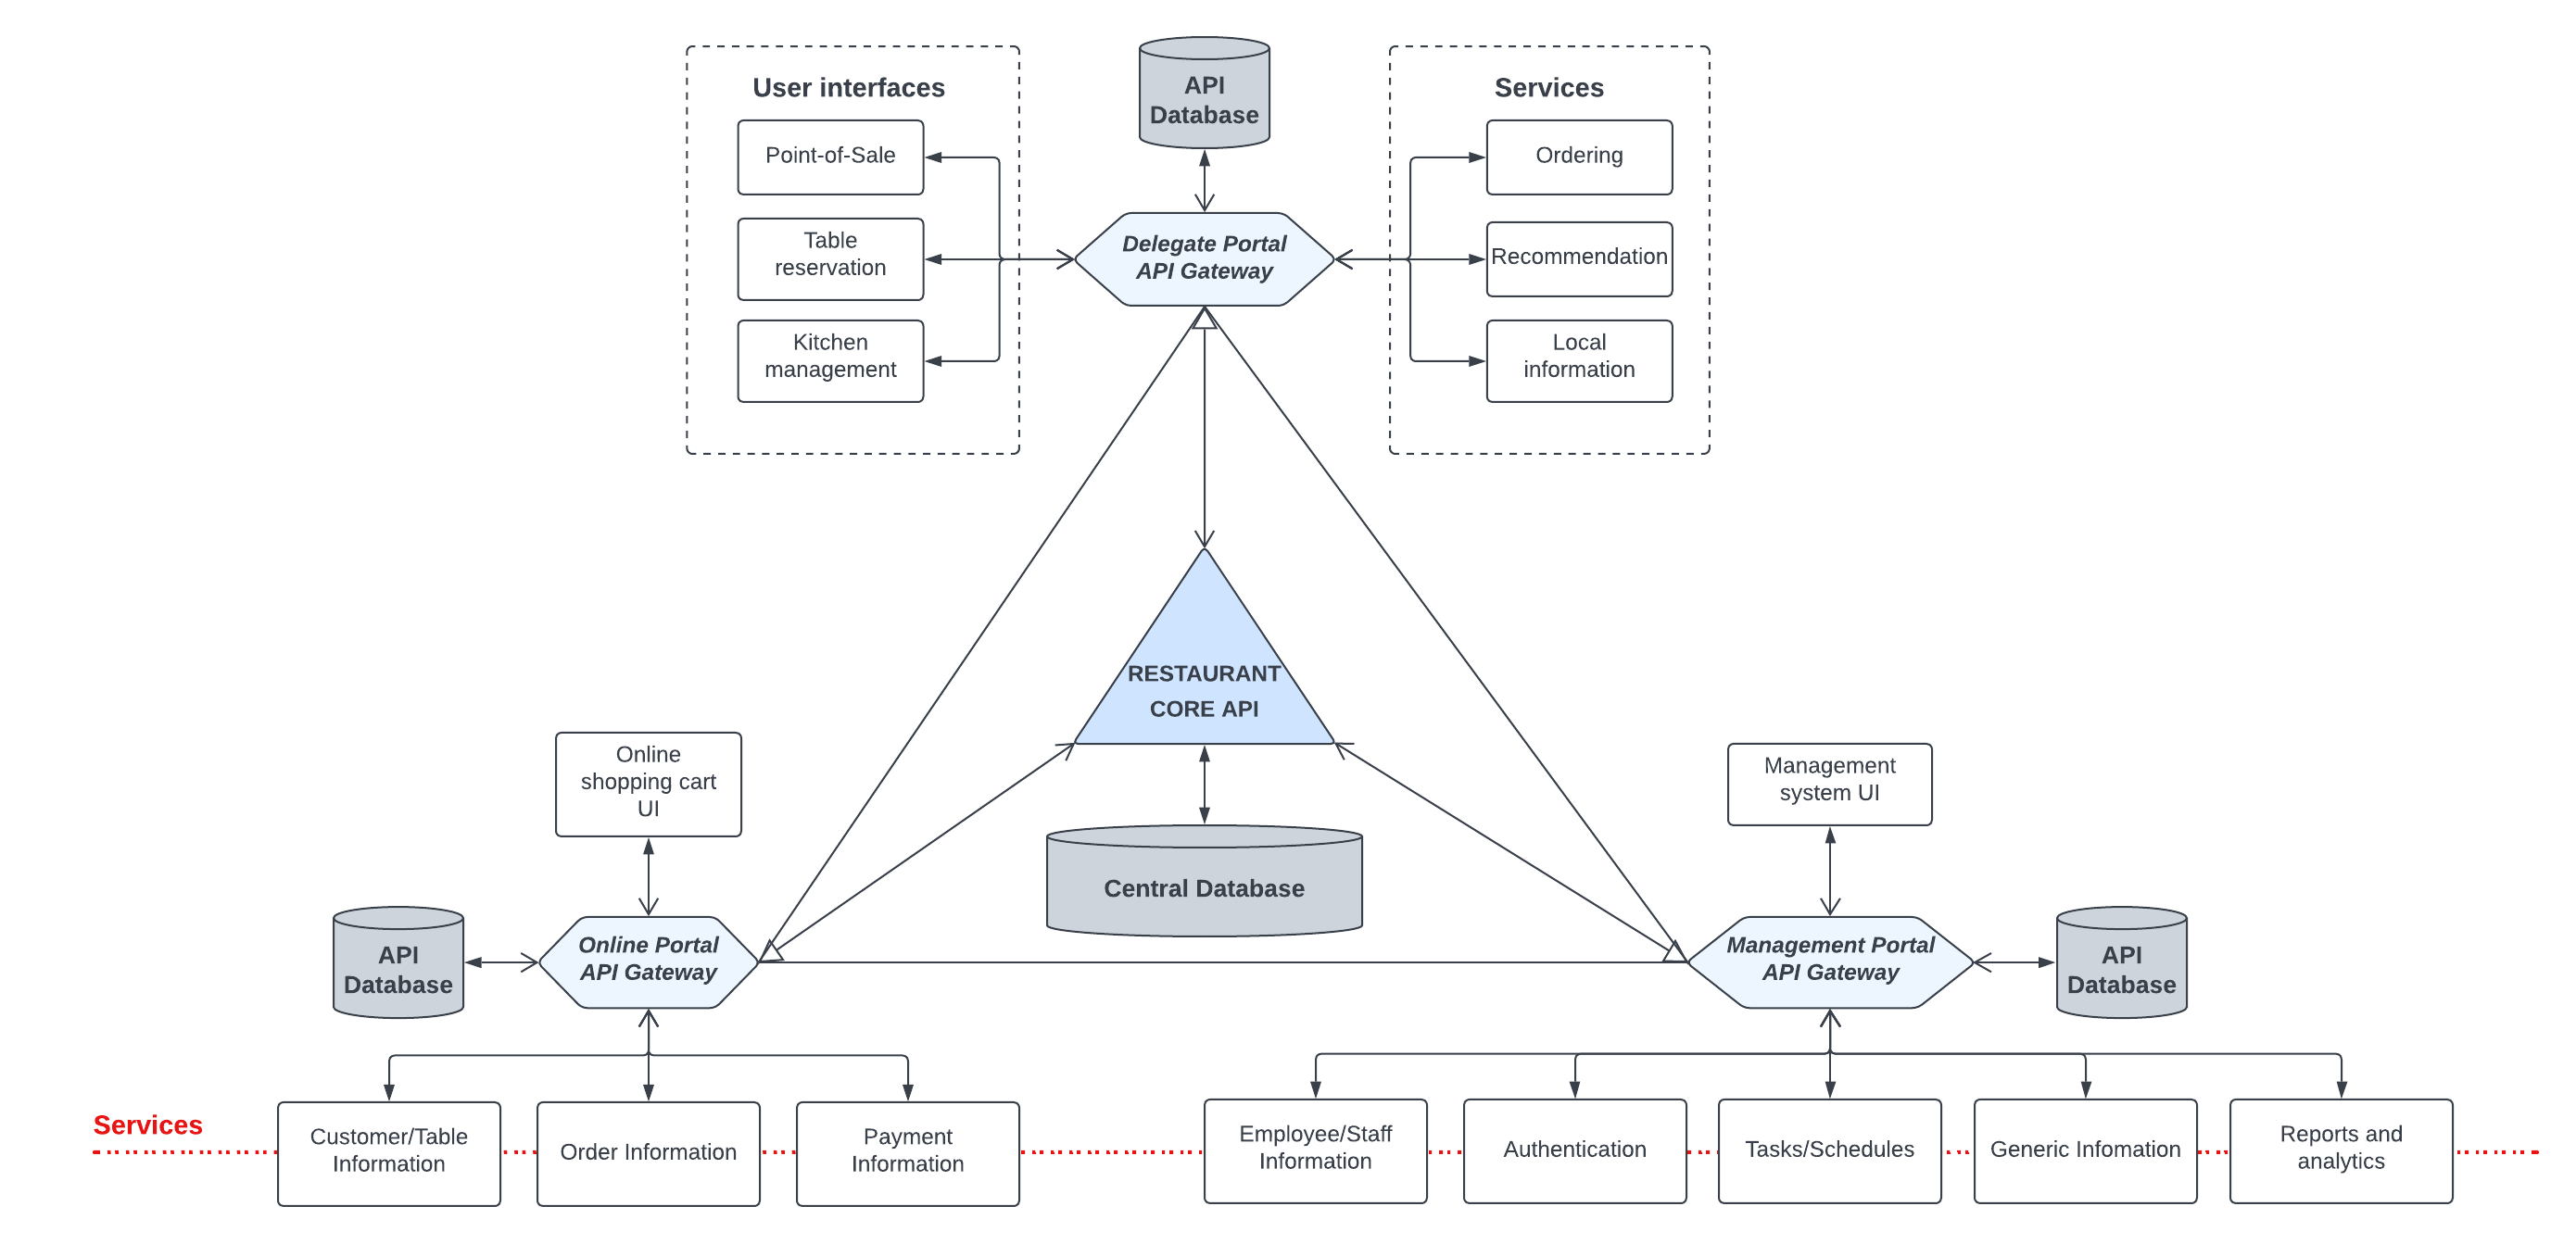
\includegraphics[width=23cm]{Cloud-native Arch.png}
	\caption{Cloud-native architecture of a restaurant POS.}
	\label{fig:archdiag}
\end{sidewaysfigure}

\noindent the rest of the API network. Provided that one or more sub-API experience malfunction or undergoes maintenance/software updates, only the branch of that API is disabled while not affecting the rest of the network. If the central API is turned off temporarily, the local sub-API databases are utilized to store their own data and sends synchronization signal to other sub-databases to keep everything updated while access to the core is limited.

\vspace{5mm}
It is virtually impossible for external attempts to directly access the database without an appropriate sub-API intervention. Regardless of compromises from sub-API and its own database, it will not affect other nodes.

\vspace{5mm}
In addition to security benefits, the architecture can be expanded to accompany more sub-APIs in the future while keeping a cohesive footprint of the nodes in the network. It is even more efficient for interaction between multiple core APIs, e.g. the restaurant system to other networks of restaurants (layered cloud-native), providing wider business opportunities.

\section{Functional requirement implementation} 

The following deployment diagram models the physical deployment of artifacts on nodes, in this case, the topology of the POS system outlines six logical components: website package, customer management, order, menu, payment and seating requirements.

\vspace{5mm}
When a user executes an order on the website, their operations are performed in a packaged online environment. One can visit the website, browse through a list of menus, make order and seating reservation, while optionally choose to sign up or sign in to their account. After everything is completed, the payment system shall be activated and can access the customer database if prompted.

\begin{sidewaysfigure}
	\centering
	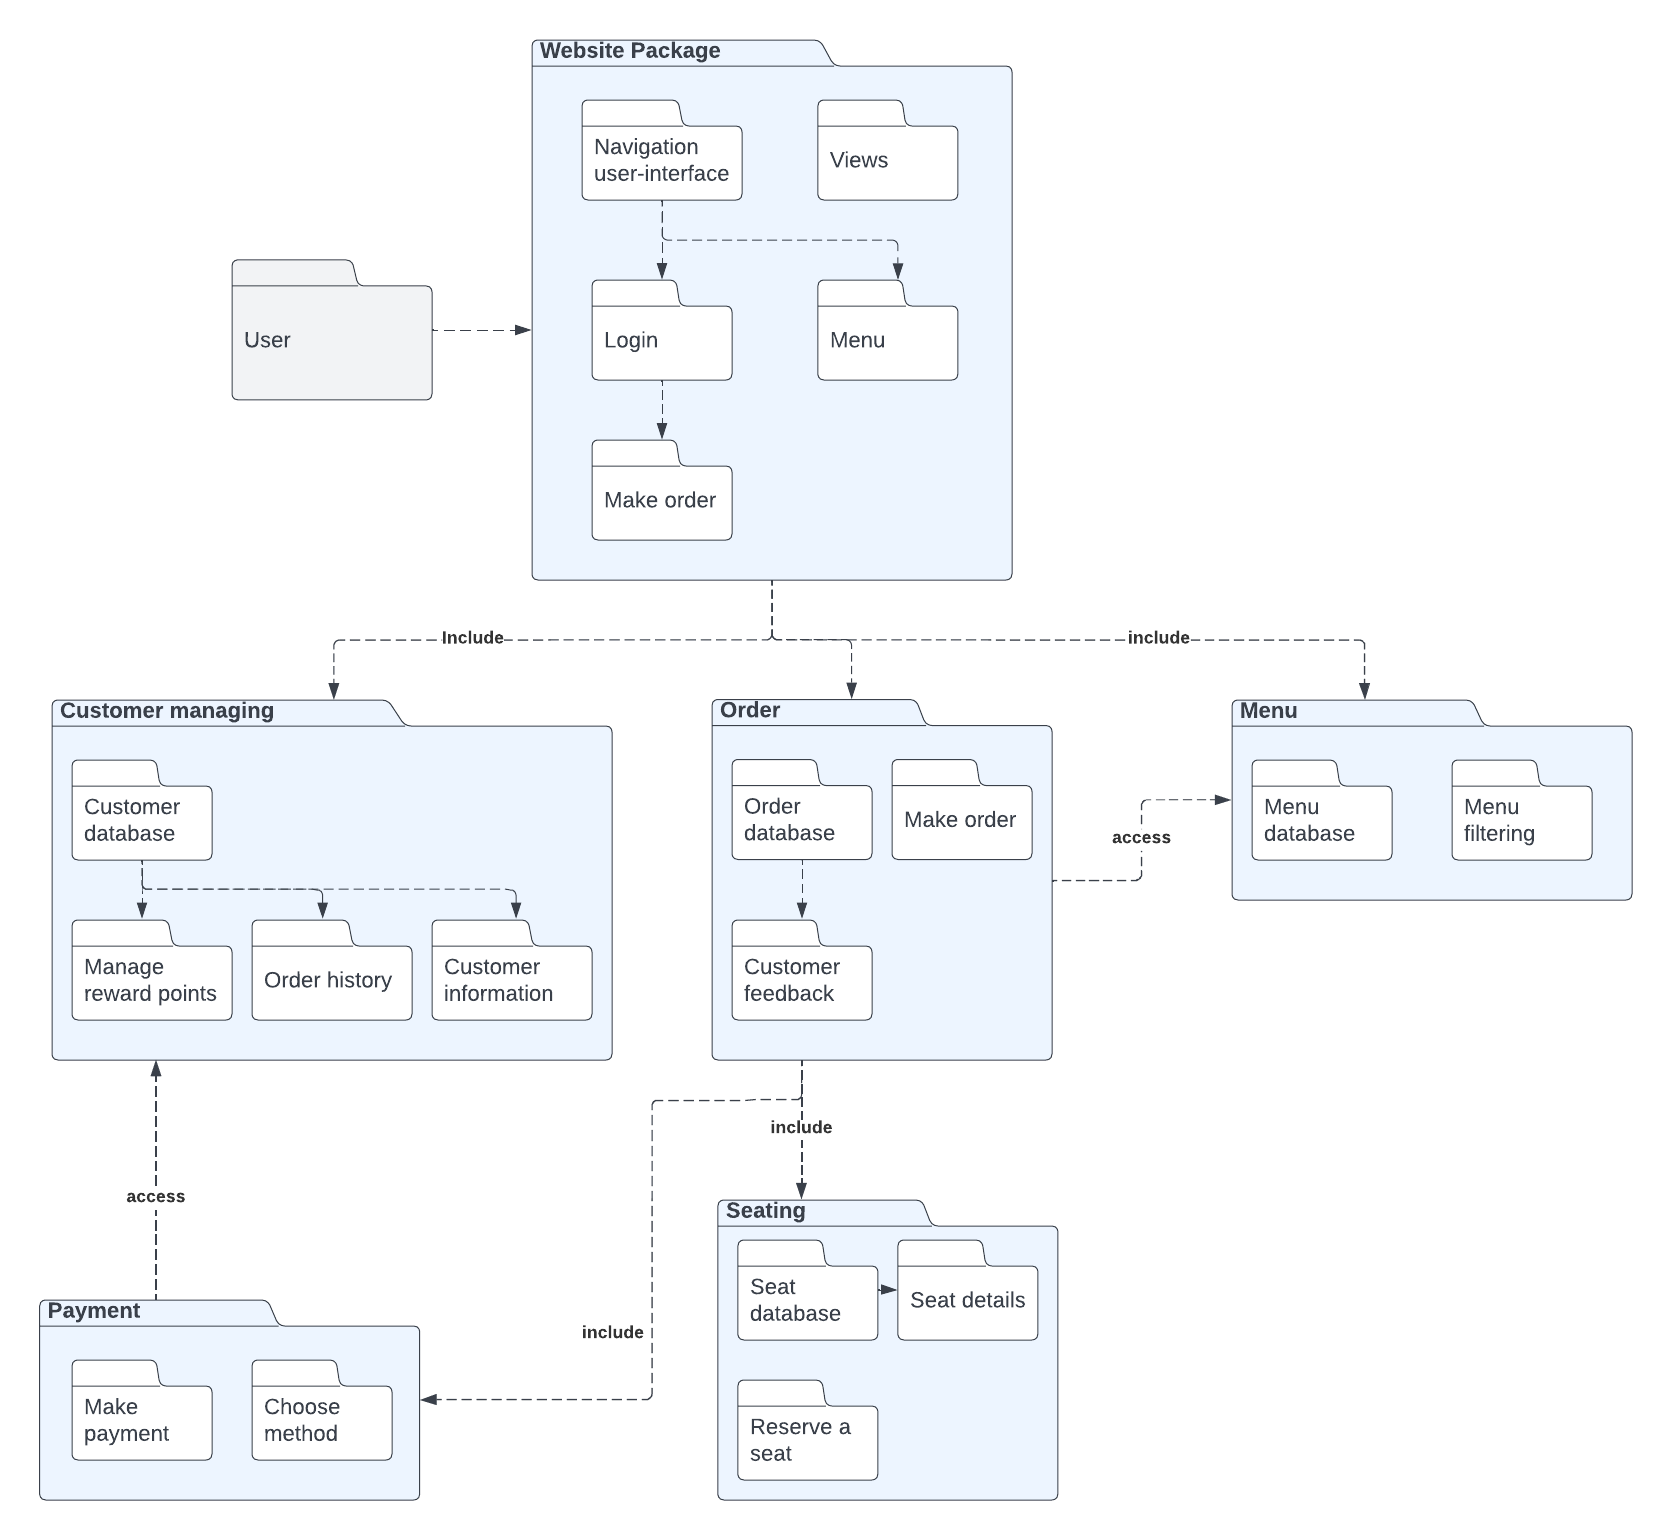
\includegraphics[width=18cm]{functrq.png}
	\caption{Deployment graph of a restaurant POS and its functional requirements.}
	\label{fig:reqdiag}
\end{sidewaysfigure}

\newpage
\thispagestyle{empty}
\vspace*{\fill}
\centering
\textit{End of report part 3}\\
\textit{This page is intentionally left blank} \\
\textit{The design and project documented in this \LaTeX is copyrighted to its correspondences in this group.}


\end{document}